
\makeatletter
\@ifundefined{standalonetrue}{\newif\ifstandalone}{}
\@ifundefined{section}{\standalonetrue}{\standalonefalse}
\makeatother
\ifstandalone
\documentclass{report}

\usepackage{textcase}
%\usepackage{hyperref}
%\hypersetup{breaklinks=true}


% Added packages
\usepackage[usenames]{color}
\usepackage{amsfonts, amsmath, amssymb, graphics}

% NOTE: bibentry MUST appear before the hyperref or build will fail
\usepackage{bibentry}
\nobibliography*
\usepackage[square,sort,comma,numbers]{natbib}
  
\usepackage{float}
\usepackage[
	hidelinks,%
    %hyperindex=true,		% Make numbers of index links as well
   	backref=page, 		% Provide page listing where refs occur in the bibliography
	%breaklinks=true,
    %colorlinks,%
    %citecolor=green,%
    %filecolor=blue,%
    %linkcolor=red,%
    %urlcolor=red, 
]{hyperref}

\usepackage{dsfont}
%%%% USEPACKAGES for MACROS %%%%%
\usepackage{algpseudocode}
\usepackage[chapter]{algorithm}
%\usepackage{caption}
\usepackage{subcaption}
\usepackage{url}

\usepackage{array}
\usepackage{arydshln}
\usepackage{multirow}
\usepackage{multicol}
%\usepackage[section]{placeins}

\usepackage[usenames,dvipsnames]{color}
%\usepackage[english]{babel}
\usepackage{tabularx}
\usepackage{soul}
\usepackage{xparse}
\usepackage{listings}
%\usepackage[normalem]{ulem}



%%%%%%%%%%%%%%%
% Show a list of items "todo" or "done" 
% USAGE: 
% \begin{todolist} 
% 	\todo Something not finished
% 	\done Something finished
% \end{todolist} 
\newenvironment{todolist}{%
  \begin{list}{}{}% whatever you want the list to be
  \let\olditem\item
  \renewcommand\item{\olditem \textcolor{red}{(TODO)}: }
  \newcommand\todo{\olditem \textcolor{red}{(TODO)}: }
   \newcommand\done{\olditem \textcolor{ForestGreen}{(DONE)}: }
}{%
  \end{list}
} 
%%%%%%%%%%%%%%%

%%%%%%%%%%%%%%%
% Show a Author's Note
% USAGE: 
% \incomplete[Optional footnote message to further clarify note]{The text which is currently not finished}
\DeclareDocumentCommand \incomplete{ o m }
{%
\IfNoValueTF {#1}
{\textcolor{red}{Incomplete: \ul{#2}}} 
{\textcolor{red}{Incomplete: \ul{#2}}\footnote{Comment: #1}}%
}
%%%%%%%%%%%%%%%



%%%%%%%%%%%%%%%
% Show a Author's Note
% USAGE: 
% \authnote[Optional footnote message to further clarify note]{The note to your readers}
\DeclareDocumentCommand \authnote { o m }
{%
\IfNoValueTF {#1}
{\textcolor{blue}{Author's Note: \ul{#2}}} 
{\textcolor{blue}{Author's Note: \ul{#2}}\footnote{Comment: #1}}%
}
%%%%%%%%%%%%%%%



%%%%%%%%%%%%%%%
% Strike out text that doesn't belong in the paper
% USAGE: 
% \strike[Optional footnote to state why it doesn't belong]{Text to strike out}
\DeclareDocumentCommand \strike { o m }
{%
\setstcolor{Red}
\IfNoValueTF {#1}
{\textcolor{Gray}{\st{#2}}} 
{\textcolor{Gray}{\st{#2}}\footnote{Comment: #1}}%
}
%%%%%%%%%%%%%%%

\definecolor{light-gray}{gray}{0.95}

\newcommand{\cbox}[3]{
\ \\
\fcolorbox{#1}{#2}{
\parbox{\textwidth}{
#3
}
}
}

% Setup an environment similar to verbatim but which will highlight any bash commands we have
\lstnewenvironment{unixcmds}[0]
{
%\lstset{language=bash,frame=shadowbox,rulesepcolor=\color{blue}}
\lstset{ %
language=sh,		% Language
basicstyle=\ttfamily,
backgroundcolor=\color{light-gray}, 
rulecolor=\color{blue},
%frame=tb, 
columns=fullflexible,
%framexrightmargin=-.2\textwidth,
linewidth=0.8\textwidth,
breaklines=true,
%prebreak=/, 
  prebreak = \raisebox{0ex}[0ex][0ex]{\ensuremath{\hookleftarrow}},
%basicstyle=\footnotesize,       % the size of the fonts that are used for the code
%numbers=left,                   % where to put the line-numbers
%numberstyle=\footnotesize,      % the size of the fonts that are used for the line-numbers
%stepnumber=2,                   % the step between two line-numbers. If it's 1 each line 
                                % will be numbered
%numbersep=5pt,                  % how far the line-numbers are from the code
showspaces=false,               % show spaces adding particular underscores
showstringspaces=false,         % underline spaces within strings
showtabs=false,                 % show tabs within strings adding particular underscores
frame=single,	                % adds a frame around the code
tabsize=2,	                % sets default tabsize to 2 spaces
captionpos=b,                   % sets the caption-position to bottom
breakatwhitespace=false,        % sets if automatic breaks should only happen at whitespace
}
} { }

% Setup an environment similar to verbatim but which will highlight any bash commands we have
\lstnewenvironment{cppcode}[1]
{
%\lstset{language=bash,frame=shadowbox,rulesepcolor=\color{blue}}
\lstset{ %
	backgroundcolor=\color{light-gray}, 
	rulecolor=\color[rgb]{0.133,0.545,0.133},
	tabsize=4,
	language=[GNU]C++,
%	basicstyle=\ttfamily,
        basicstyle=\scriptsize,
        upquote=true,
        aboveskip={1.5\baselineskip},
        columns=fullflexible,
        %framexrightmargin=-.1\textwidth,
       %framexleftmargin=6mm,
        showstringspaces=false,
        extendedchars=true,
        breaklines=true,
        prebreak = \raisebox{0ex}[0ex][0ex]{\ensuremath{\hookleftarrow}},
        frame=single,
        showtabs=false,
        showspaces=false,
        showstringspaces=false,
        numbers=left,                   % where to put the line-numbers
	numberstyle=\footnotesize,      % the size of the fonts that are used for the line-numbers
	stepnumber=4,                   % the step between two line-numbers. If it's 1 each line 
                                % will be numbered
	firstnumber=#1,
         numbersep=5pt,                  % how far the line-numbers are from the code
        identifierstyle=\ttfamily,
        keywordstyle=\color[rgb]{0,0,1},
        commentstyle=\color[rgb]{0.133,0.545,0.133},
        stringstyle=\color[rgb]{0.627,0.126,0.941},
}
} { }

% Setup an environment similar to verbatim but which will highlight any bash commands we have
\lstnewenvironment{mcode}[1]
{
\lstset{ %
	backgroundcolor=\color{light-gray}, 
	rulecolor=\color[rgb]{0.133,0.545,0.133},
	tabsize=4,
	language=Matlab,
%	basicstyle=\ttfamily,
        basicstyle=\scriptsize,
        upquote=true,
        aboveskip={1.5\baselineskip},
        columns=fullflexible,
        %framexrightmargin=-.1\textwidth,
       %framexleftmargin=6mm,
        showstringspaces=false,
        extendedchars=true,
        breaklines=true,
        prebreak = \raisebox{0ex}[0ex][0ex]{\ensuremath{\hookleftarrow}},
        frame=single,
        showtabs=false,
        showspaces=false,
        showstringspaces=false,
        numbers=left,                   % where to put the line-numbers
	numberstyle=\footnotesize,      % the size of the fonts that are used for the line-numbers
	stepnumber=4,                   % the step between two line-numbers. If it's 1 each line 
                                % will be numbered
	firstnumber=#1,
         numbersep=5pt,                  % how far the line-numbers are from the code
        identifierstyle=\ttfamily,
        keywordstyle=\color[rgb]{0,0,1},
        commentstyle=\color[rgb]{0.133,0.545,0.133},
        stringstyle=\color[rgb]{0.627,0.126,0.941},
}
} { }

\newcommand{\inputmcode}[1]{%
\lstset{ %
	backgroundcolor=\color{light-gray},  %
	rulecolor=\color[rgb]{0.133,0.545,0.133}, %
	tabsize=4, %
	language=Matlab, %
%	basicstyle=\ttfamily,
        basicstyle=\scriptsize, %
        %        upquote=true,
        aboveskip={1.5\baselineskip}, %
        columns=fullflexible, %
        %framexrightmargin=-.1\textwidth,
       %framexleftmargin=6mm,
        showstringspaces=false, %
        extendedchars=true, %
        breaklines=true, %
        prebreak = \raisebox{0ex}[0ex][0ex]{\ensuremath{\hookleftarrow}}, %
        frame=single, %
        showtabs=false, %
        showspaces=false, %
        showstringspaces=false,%
        numbers=left,                   % where to put the line-numbers
	numberstyle=\footnotesize,      % the size of the fonts that are used for the line-numbers
	stepnumber=4,                   % the step between two line-numbers. If it's 1 each line 
                                % will be numbered
         numbersep=5pt,                  % how far the line-numbers are from the code
        identifierstyle=\ttfamily, %
        keywordstyle=\color[rgb]{0,0,1}, %
        commentstyle=\color[rgb]{0.133,0.545,0.133}, %
        stringstyle=\color[rgb]{0.627,0.126,0.941} %
}
\lstinputlisting{#1}%
}

%\lstset{ %
%	backgroundcolor=\color{light-gray}, 
%	rulecolor=\color[rgb]{0.133,0.545,0.133},
%	tabsize=4,
%	language=Matlab,
%%	basicstyle=\ttfamily,
%        basicstyle=\scriptsize,
%        upquote=true,
%        aboveskip={1.5\baselineskip},
%        columns=fullflexible,
%        %framexrightmargin=-.1\textwidth,
%       %framexleftmargin=6mm,
%        showstringspaces=false,
%        extendedchars=true,
%        breaklines=true,
%        prebreak = \raisebox{0ex}[0ex][0ex]{\ensuremath{\hookleftarrow}},
%        frame=single,
%        showtabs=false,
%        showspaces=false,
%        showstringspaces=false,
%        numbers=left,                   % where to put the line-numbers
%	numberstyle=\footnotesize,      % the size of the fonts that are used for the line-numbers
%	stepnumber=4,                   % the step between two line-numbers. If it's 1 each line 
%                                % will be numbered
%	firstnumber=#1,
%         numbersep=5pt,                  % how far the line-numbers are from the code
%        identifierstyle=\ttfamily,
%        keywordstyle=\color[rgb]{0,0,1},
%        commentstyle=\color[rgb]{0.133,0.545,0.133},
%        stringstyle=\color[rgb]{0.627,0.126,0.941},
%}


\newcommand{\Laplacian}[1]{\nabla^2 #1}

% set of all nodes received and contained on GPU
\newcommand{\setAllNodes}[0]{\mathcal{G}}
% set of stencil centers on GPU
\newcommand{\setCenters}[0]{\mathcal{Q}}
% set of stencil centers with nodes in \setDepend
\newcommand{\setBoundary}[0]{\mathcal{B}}
% set of nodes received by other GPUs
\newcommand{\setDepend}[0]{\mathcal{R}}
% set of nodes sent to other GPUs
\newcommand{\setProvide}[0]{\mathcal{O}}


\newcommand{\toprule}[0]{\hline}
\newcommand{\midrule}[0]{\hline\hline}
\newcommand{\bottomrule}[0]{\hline}

\newcolumntype{C}{>{\centering\arraybackslash}b{1in}}
\newcolumntype{L}{>{\flushleft\arraybackslash}b{1.5in}}
\newcolumntype{R}{>{\flushright\arraybackslash}b{1.5in}}
\newcolumntype{D}{>{\flushright\arraybackslash}b{2.0in}}
\newcolumntype{E}{>{\flushright\arraybackslash}b{1.0in}}

\DeclareSymbolFont{AMSb}{U}{msb}{m}{n}
\DeclareMathSymbol{\N}{\mathbin}{AMSb}{"4E}
\DeclareMathSymbol{\Z}{\mathbin}{AMSb}{"5A}
\DeclareMathSymbol{\R}{\mathbin}{AMSb}{"52}
\DeclareMathSymbol{\Q}{\mathbin}{AMSb}{"51}
\DeclareMathSymbol{\PP}{\mathbin}{AMSb}{"50}
\DeclareMathSymbol{\I}{\mathbin}{AMSb}{"49}
%\DeclareMathSymbol{\C}{\mathbin}{AMSb}{"43}

%%%%%% VECTOR NORM: %%%%%%%
\newcommand{\vectornorm}[1]{\left|\left|#1\right|\right|}
\newcommand{\vnorm}[1]{\left|\left|#1\right|\right|}
\newcommand{\by}[0]{\times}
\newcommand{\vect}[1]{\mathbf{#1}}
%\newcommand{\mat}[1]{\mathbf{#1}} 

%\renewcommand{\vec}[1]{ \textbf{#1} }
%%%%%%%%%%%%%%%%%%%%%%

%%%%%%% THM, COR, DEF %%%%%%%
%\newtheorem{theorem}{Theorem}[section]
%\newtheorem{lemma}[theorem]{Lemma}
%\newtheorem{proposition}[theorem]{Proposition}
%\newtheorem{corollary}[theorem]{Corollary}
%\newenvironment{proof}[1][Proof]{\begin{trivlist}
%\item[\hskip \labelsep {\bfseries #1}]}{\end{trivlist}}
%\newenvironment{definition}[1][Definition]{\begin{trivlist}
%\item[\hskip \labelsep {\bfseries #1}]}{\end{trivlist}}
%\newenvironment{example}[1][Example]{\begin{trivlist}
%\item[\hskip \labelsep {\bfseries #1}]}{\end{trivlist}}
%\newenvironment{remark}[1][Remark]{\begin{trivlist}
%\item[\hskip \labelsep {\bfseries #1}]}{\end{trivlist}}
%\newcommand{\qed}{\nobreak \ifvmode \relax \else
%      \ifdim\lastskip<1.5em \hskip-\lastskip
%      \hskip1.5em plus0em minus0.5em \fi \nobreak
%      \vrule height0.75em width0.5em depth0.25em\fi}
%%%%%%%%%%%%%%%%%%%%%%

%
%\usepackage[algochapter]{algorithm2e}
%\usepackage[usenames]{color}
% colors to show the corrections
\newcommand{\red}[1]{\textbf{\textcolor{red}{#1}}}
\newcommand{\blue}[1]{\textbf{\textcolor{blue}{#1}}}
\newcommand{\cyan}[1]{\textbf{\textcolor{cyan}{#1}}}
\newcommand{\green}[1]{\textbf{\textcolor{green}{#1}}}
\newcommand{\magenta}[1]{\textbf{\textcolor{magenta}{#1}}}
\newcommand{\orange}[1]{\textbf{\textcolor{orange}{#1}}}
%%%%%%%%%% DK DK
% comments between authors
\newcommand{\toall}[1]{\textbf{\green{@@@ All: #1 @@@}}}
\newcommand{\toevan}[1]{\textbf{\red{*** Evan: #1 ***}}}
%\newcommand{\toevan}[1]{}  % USE FOR FINAL VERSION
\newcommand{\toe}[1]{\textbf{\red{*** Evan: #1 ***}}}
\newcommand{\tog}[1]{\textbf{\blue{*** Gordon: #1 ***}}}
%\newcommand{\togordon}[1]{\textbf{\blue{*** Gordon: #1 ***}}}
\renewcommand{\ge}[3]{{\textcolor{blue}{*** \textbf{Gordon:}\strike{#1} #2 ***}}\red{(#3)}}
\renewcommand{\ge}[3]{{\textcolor{blue}{#2}}}
\renewcommand{\ge}[3]{{\textcolor{Red}{#2}}}
\newcommand{\eb}[3]{{\textcolor{Red}{*** \textbf{Evan:}\strike{#1} #2 ***}}\red{(#3)}}
\renewcommand{\eb}[3]{{{\textcolor{Red}{#2}}}}
%\def\ge#1#2#3{}{\textbf{\blue{*** Gordon: #2 ***}}}{(#3)}
\newcommand{\gee}[1]{{\bf{\blue{{\em #1}}}}}
\newcommand{\old}[1]{}
\newcommand{\del}[1]{***#1*** }



% \DeclareMathOperator{\Sample}{Sample}
%\let\vaccent=\v % rename builtin command \v{} to \vaccent{}
%\renewcommand{\vec}[1]{\ensuremath{\mathbf{#1}}} % for vectors
\newcommand{\gv}[1]{\ensuremath{\mbox{\boldmath$ #1 $}}} 
% for vectors of Greek letters
\newcommand{\uv}[1]{\ensuremath{\mathbf{\hat{#1}}}} % for unit vector
\newcommand{\abs}[1]{\left| #1 \right|} % for absolute value
\newcommand{\avg}[1]{\left< #1 \right>} % for average
\let\underdot=\d % rename builtin command \d{} to \underdot{}
\renewcommand{\d}[2]{\frac{d #1}{d #2}} % for derivatives
\newcommand{\dd}[2]{\frac{d^2 #1}{d #2^2}} % for double derivatives
\newcommand{\pd}[2]{\frac{\partial #1}{\partial #2}} 
% for partial derivatives
\newcommand{\pdd}[2]{\frac{\partial^2 #1}{\partial #2^2}} 
\newcommand{\pdda}[3]{\frac{\partial^2 #1}{\partial #2 \partial #3}} 
% for double partial derivatives
\newcommand{\pdc}[3]{\left( \frac{\partial #1}{\partial #2}
 \right)_{#3}} % for thermodynamic partial derivatives
\newcommand{\ket}[1]{\left| #1 \right>} % for Dirac bras
\newcommand{\bra}[1]{\left< #1 \right|} % for Dirac kets
\newcommand{\braket}[2]{\left< #1 \vphantom{#2} \right|
 \left. #2 \vphantom{#1} \right>} % for Dirac brackets
\newcommand{\matrixel}[3]{\left< #1 \vphantom{#2#3} \right|
 #2 \left| #3 \vphantom{#1#2} \right>} % for Dirac matrix elements
\newcommand{\grad}[1]{\gv{\nabla} #1} % for gradient
\let\divsymb=\div % rename builtin command \div to \divsymb
\renewcommand{\div}[1]{\gv{\nabla} \cdot #1} % for divergence
\newcommand{\curl}[1]{\gv{\nabla} \times #1} % for curl
\let\baraccent=\= % rename builtin command \= to \baraccent
\renewcommand{\=}[1]{\stackrel{#1}{=}} % for putting numbers above =
\newcommand{\diffop}[1]{\mathcal{L}#1}
\newcommand{\boundop}[1]{\mathcal{B}#1}
\newcommand{\rvec}[0]{{\bf r}}

\newcommand{\Interior}[0]{\Omega}
\newcommand{\domain}[0]{\Omega}
%\newcommand{\Boundary}[0]{\partial \Omega}
\newcommand{\Boundary}[0]{\Gamma}

\newcommand{\on}[1]{\hskip1.5em \textrm{ on } #1}

\newcommand{\gemm}{\texttt{GEMM}}
\newcommand{\trmm}{\texttt{TRMM}}
\newcommand{\gesvd}{\texttt{GESVD}}
\newcommand{\geqrf}{\texttt{GEQRF}}


\newcommand{\minitab}[2][l]{\begin{tabular}{#1}#2\end{tabular}}
\newcommand{\comm}[1]{\textcolor{red}{\textit{#1}}}

\newcommand{\nfrac}[2]{
\nicefrac{#1}{#2}
%\frac{#1}{#2}
}

\usepackage{xparse}
\usepackage{soul}


%%%%%%%%%%%%%%%
% Show a Author's Note
% USAGE: 
% \incomplete[Optional footnote message to further clarify note]{The text which is currently not finished}
\DeclareDocumentCommand \incomplete{ o m }
{%
\IfNoValueTF {#1}
{\textcolor{red}{Incomplete: \ul{#2}}} 
{\textcolor{red}{Incomplete: \ul{#2}}\footnote{Comment: #1}}%
}
%%%%%%%%%%%%%%%



%%%%%%%%%%%%%%%
% Show a Author's Note
% USAGE: 
% \authnote[Optional footnote message to further clarify note]{The note to your readers}
\DeclareDocumentCommand \authnote { o m }
{%
\IfNoValueTF {#1}
{\textcolor{blue}{Author's Note: \ul{#2}}} 
{\textcolor{blue}{Author's Note: \ul{#2}}\footnote{Comment: #1}}%
}
%%%%%%%%%%%%%%%



%%%%%%%%%%%%%%%
% Strike out text that doesn't belong in the paper
% USAGE: 
% \strike[Optional footnote to state why it doesn't belong]{Text to strike out}
\DeclareDocumentCommand \strike { o m }
{%
\setstcolor{red}
\IfNoValueTF {#1}
{\textcolor{Gray}{\st{#2}}} 
{\textcolor{Gray}{\st{#2}}\footnote{Comment: #1}}%
}
%%%%%%%%%%%%%%%



%
% colors to show the corrections
\newcommand{\red}[1]{\textbf{\textcolor{red}{#1}}}
\newcommand{\blue}[1]{\textbf{\textcolor{blue}{#1}}}
\newcommand{\cyan}[1]{\textbf{\textcolor{cyan}{#1}}}
\newcommand{\green}[1]{\textbf{\textcolor{green}{#1}}}
\newcommand{\magenta}[1]{\textbf{\textcolor{magenta}{#1}}}
\newcommand{\orange}[1]{\textbf{\textcolor{orange}{#1}}}
%%%%%%%%%% DK DK
% comments between authors
\newcommand{\toall}[1]{\textbf{\green{@@@ All: #1 @@@}}}
\newcommand{\toevan}[1]{\textbf{\red{*** Evan: #1 ***}}}
%\newcommand{\toevan}[1]{}  % USE FOR FINAL VERSION
\newcommand{\toe}[1]{\textbf{\red{*** Evan: #1 ***}}}
\newcommand{\tog}[1]{\textbf{\blue{*** Gordon: #1 ***}}}
%\newcommand{\togordon}[1]{\textbf{\blue{*** Gordon: #1 ***}}}
\renewcommand{\ge}[3]{{\textcolor{blue}{*** \textbf{Gordon:}\strike{#1} #2 ***}}\red{(#3)}}
\renewcommand{\ge}[3]{{\textcolor{blue}{#2}}}
\renewcommand{\ge}[3]{{\textcolor{red}{#2}}}
\newcommand{\eb}[3]{{\textcolor{red}{*** \textbf{Evan:}\strike{#1} #2 ***}}\red{(#3)}}
\renewcommand{\eb}[3]{{{\textcolor{red}{#2}}}}
%\def\ge#1#2#3{}{\textbf{\blue{*** Gordon: #2 ***}}}{(#3)}
\newcommand{\gee}[1]{{\bf{\blue{{\em #1}}}}}
\newcommand{\old}[1]{}
\newcommand{\del}[1]{***#1*** }



% Rename  this file          misc_mac.tex
%----------------------------------------------------------------------
%%%%%%%%%%%%%%%%%%%%%%%%%%%%%%%%%%%%%%%%%%%%%%%%%%%%%%%%%%%%%%%%%%%%%%%%%%%%%%%
%
%	Math Symbols   Math Symbols   Math Symbols   Math Symbols   
%
%%%%%%%%%%%%%%%%%%%%%%%%%%%%%%%%%%%%%%%%%%%%%%%%%%%%%%%%%%%%%%%%%%%%%%%%%%%%%%%
\def\pmb#1{\setbox0=\hbox{$#1$}%
	\kern-.025em\copy0\kern-\wd0
	\kern.05em\copy0\kern-\wd0
	\kern-.025em\raise.0433em\box0}
\def\pmbf#1{\pmb#1}
\def\bfg#1{\pmb#1}

% BETTER VALUES FOR AUTOMATIC FIGURE PLACEMENT THAN THOSE PROVIDED BY 
% LATEX DEFAULTS.

\renewcommand{\textfloatsep}{1ex}
\renewcommand{\floatpagefraction}{0.9}
\renewcommand{\intextsep}{1ex}
\renewcommand{\topfraction}{.9}
\renewcommand{\bottomfraction}{.9}
\renewcommand{\textfraction}{.1}

% #1  position of floating figure (h|t|b|p)
% #1  EPS postscript file
% #2  size
% #3  caption

%usage of newfig:
%  \newfig{file.ps}{3in}{Fig1: this is a figure}

\input{epsf}
\def\newfig#1#2#3{
  \begin{figure}[htbp]
  \vspace{1ex}
  \setlength{\epsfxsize}{#2}
  \centerline{\epsfbox{#1}}
  \vspace{-.1in}\caption{\small #3}\break\vspace{.2in}
  \label{#1}
  \end{figure}
}

%usage of newfigtwo: 2 figures, vertically stacked
% \newfig
%	{file1.ps}
%	{file2.ps}
%	{width}
%	{vertical space}
%	{Caption}

\def\newfigtwo#1#2#3#4#5{
  \begin{figure}[htbp]
  \vspace{1ex}
  \setlength{\epsfxsize}{#3}
  \centerline{\epsfbox{#1}}
  \vspace{#4}
  \setlength{\epsfxsize}{#3}
  \centerline{\epsfbox{#2}}
  \vspace{-.1in}\caption{\small #5}\break\vspace{.2in}
  \label{#1}
  \end{figure}
}

\def\newfigh#1#2#3#4{  % add height specification
  \begin{figure}[htbp]
  \vspace{1ex}
  \setlength{\epsfxsize}{#2}
  \setlength{\epsfysize}{#4}
  \centerline{\epsfbox{#1}}
  \vspace{-.1in}\caption{\small #3}\break\vspace{.2in}
  \label{#1}
  \end{figure}
}

\def\herefig#1#2#3{
  \begin{figure}[h]
  \setlength{\epsfxsize}{#2}
  \centerline{\epsfbox{#1}}
  \caption{\small #3}
  \label{#1}
  \end{figure}
}

\def\etal{{{\em et~al.\,\,}}}
\def\note#1{\\ =====#1===== \\}
\def\FBOX#1{\ \\ \fbox{\begin{minipage}{5in}#1\end{minipage}}\\ }
\newcount\sectionno     \sectionno=0
\newcount\eqnum         \eqnum=0
\def\addeqno{\global\advance \eqnum by  1 }
\def\subeqno{\global\advance \eqnum by -1 }
%\def\eqn{\addeqno \eqno \hbox{(\number\sectionno.\number\eqnum)} }

\def\tildetilde#1{\tilde{\tilde{#1}}}
\def\barbar#1{\overbar{\overbar{#1}}}

\def\vsp#1{\vspace{#1 ex}}
\def\fpar{\hspace{\parindent}}
%
%  \pf : 2 arguments: numerator and denominator of partial derivative
%
\def\pf#1#2{{\frac{\partial{#1}}{\partial{#2}}}}
\def\pfs#1#2{{\partial_{#2}{#1}}}
\def\pftwo#1#2{{\frac{\partial^2{#1}}{\partial{#2}^2}}}
\def\pfxx#1#2{{\frac{\partial^2{#1}}{\partial{#2}^2}}}
%\def\pfxy#1#2{{\frac{\partial^2{#1}}{\partial{#2}\partial{#3}}}}
\def\pfn#1#2#3{{\frac{\partial^{#1}{#2}}{\partial{#3}^{#1}}}}
\def\df#1#2{{\frac{d{#1}}{d{#2}}}}
\def\dfn#1#2#3{{\frac{d^{#1}{#2}}{d{#3}^{#1}}}}
\def\Dt#1#2{\frac{D#1}{D#2}}
\def\dt#1#2{\frac{d#1}{d#2}}
\def\bld#1{{\bf #1}}
\def\pfp#1#2#3{\pf{}{#3}{\left(\frac{#1}{#2}\right)}}

\def\norm#1{\|#1\|}

%
% Graphic characters  (\dot already defined by TeX/LateX)
%
\def\dash{\rule[1.5pt]{2mm}{.3mm}\HS{.9mm}}
\def\dott{\rule[1.5pt]{.7mm}{.3mm}\HS{.7mm}}
\def\dashline{\dash\dash\dash}
\def\dotline{\dott\dott\dott\dott\dott\dott}
\def\dashdotline{\dash$\cdot$\HS{.9mm}\dash}
\def\solidline{\rule[2pt]{7mm}{.3mm}}
% 
% overcircle
%
\def\ovcircle#1{\buildrel{\circ}\over{#1}}
%\def\below#1#2{\buildrel{#2}\under{#1}}
%\def\above#1#2{\buildrel{#2}\over{#1}}
%
%  big parenthesis and brackets
%
\def\bigpar#1#2{{\left(\frac{#1}{#2}\right)}}
\def\bigbra#1#2{{\left\[\frac{#1}{#2}\right\]}}

\def\Lp{\left(}
\def\Rp{\right)}
\def\Lb{\left[}
\def\Rb{\right]}
\def\Ln{\left\langle}
\def\Rn{\right\rangle}
\def\Ld{\left.}
\def\Rd{\right.}
\def\Lv{\left|}
\def\Rv{\right|}
\def\Lbr{\left|}
\def\Rbr{\right|}
\def\lng{\langle}
\def\rng{\rangle}
\def\Lc{\left\{}
\def\Rc{\right\}}
%%% %

% Cannot be handled by Lyx
%\def\[{{[}}
%\def\]{{]}}

%
\def\eol{\nonumber \\}
\def\eolnonb{\nonumber\\}
\def\eolnb{\\}
\def\nonb{\nonumber}
\def\be{\begin{equation}}
\def\ee{\end{equation}}
\def\BEQNA{\begin{eqnarray}}
\def\EEQNA{\end{eqnarray}}
\def\eqa{&=&}
\def\beqna{\begin{eqnarray}}
\def\eeqna{\end{eqnarray}}
\def\bverb{\begin{verbatim}}
\def\everb{\end{verbatim}}
\def\VERB#1{\bverb #1 \everb}
\def\btbl{\begin{tabular}}
\def\etbl{\end{tabular}}
\def\bmini{\begin{minipage}[t]{5.5in}}
\def\emini{\end{minipage}}
\def\parray#1#2{\left(\begin{array}{#1}#2\end{array}\right)}
\def\barray#1#2{\left[\begin{array}{#1}#2\end{array}\right]}
\def\carray#1#2{\left\{\begin{array}{#1}#2\end{array}\right.}
\def\darray#1#2{\left|\begin{array}{#1}#2\end{array}\right|}

\def\BEGTABLE#1{\begin{table}[hbt]\vspace{2ex}\begin{center}\bmini\centering\btbl{#1}}
\def\ENDTABLE#1#2{\etbl\caption[#1]{#2}\EMINI\end{center}\vspace{2ex}\end{table}}

\def\bfltbl#1{\begin{table}[hbt]\vspace{2ex}\begin{center}\bmini\centering\btbl{#1}}
\def\efltbl#1#2{\etbl\caption[#1]{#2}\emini\end{center}\vspace{2ex}\end{table}}
\def\mcol{\multicolumn}
%
%  label equations with (#)
%
\def\reff#1{(\ref{#1})}
%
%  macros borrowed from viewgraph package
%

\newenvironment{LETTRS}[3]{\begin{letter}{#1}
\input{origin}\opening{Dear #2:}\input{#3}\closing{Sincerely yours,}\end{letter}}{\clearpage}

\newenvironment{VIEW}[1]{{\BC\Huge\bf #1 \EC}\LARGE\VS{.05in}}{\clearpage}

\def\RM#1{\rm{#1\ }}
\def\BV{\begin{VIEW}}
\def\EV{\end{VIEW}}

\def\NI{\noindent}

\def\VS{\vspace*}
\def\HS{\hspace*}
\def\IT{\item}

\def\BARR{\begin{array}}
\def\EARR{\end{array}}

\def\BPARR{\left(\begin{array}}
\def\EPARR{\end{array}\right)}

\def\BDET{\left|\begin{array}}
\def\EDET{\end{array}\right|}

\def\BDF{\begin{definition}}
\def\EDF{\end{definition}}

\def\BSU{\begin{block}{Summary}}
\def\ESU{\end{block}}

\def\BEX{\begin{example}}
\def\EEX{\end{example}}

\def\BTH{\begin{theorem}}
\def\ETH{\end{theorem}}

\def\BCO{\begin{corollary}}
\def\ECO{\end{corollary}}

\def\BPROOF{\begin{proof}}
\def\EPROOF{\end{proof}}

\def\BLM{\begin{lemma}}
\def\ELM{\end{lemma}}

\def\BEQ{\begin{equation}}
\def\EEQ{\end{equation}}

\def\BEQNNB{$$}
\def\EEQNNB{$$}

\def\BE{\begin{enumerate}}
\def\EE{\end{enumerate}}

\def\BD{\begin{description}}
\def\ED{\end{description}}

\def\BI{\begin{itemize}}
\def\EI{\end{itemize}}

\def\BC{\begin{center}}
\def\EC{\end{center}}

\def\BFIG{\begin{figure}}
\def\EFIG{\end{figure}}

\def\BTABB{\begin{tabbing}}
\def\ETABB{\end{tabbing}}

\def\BMINI{\begin{minipage}}
\def\EMINI{\end{minipage}}

\def\BTABLE{\begin{table}}
\def\ETABLE{\end{table}}

\def\BTABUL{\begin{tabular}}
\def\ETABUL{\end{tabular}}

\def\MCOL{\multicolumn}
\def\UL{\underline}
\def\ULL#1{\UL{\UL{#1}}}

\def\BDOC{\begin{document}}
\def\EDOC{\end{document}}

\def\EM#1{{\em #1\/}}
\def\FN{\footnote}

% Courtesy of Ugo Piomelli

\def\latexfig #1 #2 #3 #4 #5 {\ \vfill
\hfill\hbox to 0.05in{\vbox to #3truein{
         \special{psfile="#1" angle=270 hscale=100 
                  hoffset=#4 voffset=#5 vscale=100} }\hfill}
\hfill\vspace{-0.1in}        }

% #1 is the .ps filename
% #2 is not used in the present version
% #3 is the size of the white space left above the caption (in inches)
% #4 is the horizontal offset from some unknown reference point.
%    It is in 1/72 of an inch and is positive to the right.
% #5 is the vertical offset from some unknown reference point.
%    It is in 1/72 of an inch and is positive upwards.


\newcommand{\mathsym}[1]{{}}
\newcommand{\unicode}[1]{{}}
\newcommand{\ep}{\epsilon}
\newcommand{\vv}{\mathbf{v}}
\newcommand{\vu}{\mathbf{u}}
\newcommand{\vx}{\mathbf{x}}

\newcommand{\Laplacian}[1]{\nabla^2 #1}
\newcommand{\LaplaceBeltrami}[1]{\Delta_S #1}

% set of all nodes received and contained on GPU
\newcommand{\setAllNodes}[0]{\mathcal{G}}
% set of stencil centers on GPU
\newcommand{\setCenters}[0]{\mathcal{Q}}
% set of stencil centers with nodes in \setDepend
\newcommand{\setBoundary}[0]{\mathcal{B}}
% set of nodes received by other GPUs
\newcommand{\setDepend}[0]{\mathcal{R}}
% set of nodes sent to other GPUs
\newcommand{\setProvide}[0]{\mathcal{O}}





\usepackage{tabularx} 
\newcolumntype{C}{>{\centering\arraybackslash}b{1in}}
\newcolumntype{L}{>{\flushleft\arraybackslash}b{1.5in}}
\newcolumntype{R}{>{\flushright\arraybackslash}b{1.5in}}
\newcolumntype{D}{>{\flushright\arraybackslash}b{2.0in}}
\newcolumntype{E}{>{\flushright\arraybackslash}b{1.0in}}


 


%\usepackage{xcolor}

%\usepackage{refcheck}
% Sepia
%\definecolor{myBGcolor}{HTML}{F6F0D6}
%\definecolor{myTextcolor}{HTML}{4F452C}
% Dark
%\definecolor{myBGcolor}{HTML}{3E3535}
%\definecolor{myTextcolor}{HTML}{CFECEC}
%\color{myTextcolor}
%\pagecolor{myBGcolor}
 

\begin{document}
\fi

\chapter{Numerical Validation} 

\label{chap:explicit_implicit_pdes}
%\label{sec:validation}



\subsection{CVT epsilon tests}

\cite{FlyerLehto11} consider epsilon as a function of the number of nodes on the sphere. However, this assumption requires nodes to be distributed as MD nodes. When we apply the same functions to CVTs of larger problems we get varying results. The subtle perturbations in nodes 

\hl{test on icosahedral grid}

\hl{function based on min enclosing circle instead. Will be finer tuned to the grid. if nodes are uniform in stencil and stencil size locked then the only things that can influence epsilon and conditioning is the enclosing circle radius.}


\section{Parabolic} 

Include figure tracking max temperature and min temperature. If we have zero flux conditions then they should average out. If we have Dirichlet BCs the temperature will converge to 0. 



\section{Hyperbolic} 

Here, we present the first results in the literature for parallelizing RBF-FDs on multi-CPU and multi-GPU architectures for solving PDEs. 
 To verify our multi-CPU, single GPU and multi-GPU implementations, two hyperbolic PDEs on the surface of the sphere are tested: 1) vortex roll-up \cite{NairTransport05, NairJablonowski08} and 2) solid body rotation \cite{JakobChien1995}. These tests were chosen since they are not only standard in the numerical literature, but also
for the development of RBFs in solving PDEs on the sphere \cite{FlyerWright07, Fornberg2008, FlyerLehto10, Fornberg2011a}. Although any `approximately evenly' distributed nodes on the sphere would suffice for our purposes, maximum determinant (MD) node distributions on the sphere are used (see \cite{Sloan2003} for details) in order to be consistent with previously published results (see e.g., \cite{FlyerWright07} and \cite{FornbergLehto11}). Node sets from 1024 to 27,556 are considered with stencil sizes ranging from 17 to 101.

All results in this section are produced by the single-GPU implementation. Multi-CPU and multi-GPU implementations are verified to produce these same results. Synchronization of the solution at each time-step and the use of double precision on both the CPU and GPU ensure consistent results regardless of the number and/or choice of CPU vs GPU. Eigenvalues are computed on the CPU by the Armadillo library \cite{armadillo2010}.

\subsection{Vortex Rollup}
\label{sec:numerical_validation}
The first test case demonstrates vortex roll-up of a fluid on the surface of a unit sphere. An angular velocity field causes the initial condition to spin into two diametrically opposed but stationary vortices.

The governing PDE in latitude-longitude coordinates, $(\theta,\lambda)$, is
\begin{equation}
\pd{h}{t} + \frac{u}{\cos \theta} \pd{h}{\lambda} = 0
\label{eq:vortex}
\end{equation}
where the velocity field, $u$, only depends on latitude and is given by
\begin{equation*}
u  = \omega(\theta) \cos \theta.
\end{equation*}
Note that the $\cos \theta$ in $u$ and $1/\cos{\theta}$ in (\ref{eq:vortex}) cancel in the analytic formulation, so the discrete operator approximates $\omega(\theta) \pd{}{\lambda}$. 

Here, $\omega(\theta)$ is the angular velocity component given by
\begin{equation*}
\omega(\theta) =
\begin{cases}
\frac{3\sqrt{3}}{2 \rho(\theta)} \mathrm{sech}^{2}(\rho(\theta)) \mathrm{tanh}(\rho(\theta)) & \rho(\theta) \neq 0 \\
0 & \rho(\theta) = 0
\end{cases}
\end{equation*}
where $\rho(\theta) = \rho_0 \cos \theta$ is the radial distance of the vortex with $\rho_0=3$. The exact solution to (\ref{eq:vortex}) at non-dimensional time $t$ is
\begin{equation*}
h(\lambda, \theta, t) = 1 - \mathrm{tanh}\left( \frac{\rho(\theta)}{\gamma} \sin(\lambda - \omega(\theta) t) \right),
\end{equation*}
where $\gamma$ defines the width of the frontal zone.

From a method of lines approach, the discretized version of (\ref{eq:vortex}) is
\begin{equation}
%\pd{\mathbf{h}}{t} = - \text{diag}(\omega(\theta)) D_\lambda \mathbf{h}.
\d{\mathbf{h}}{t} = - \text{diag}(\omega(\theta)) D_\lambda \mathbf{h}.
\label{eq:vortex_matrix_form}
\end{equation}
where $D_\lambda$ is the DM containing the RBF-FD weights that approximate $\pd{}{\lambda}$ at each node on the sphere.

For stability, hyperviscosity is added to the right hand side of (\ref{eq:vortex_matrix_form}) in the form given in (\ref{eq:evaluation_with_hyperviscosity}). The scaling parameter $\gamma_c$ and the order of hyperviscosity $k$ are given in
Table~\ref{tbl:vortex_hv_params}. The goal when choosing $k$ is to damp the higher spurious eigenmodes of $\text{diag}(\omega(\theta)) D_\lambda$ while leaving the lower physical modes that can be resolved by the stencil intact. In this process, the eigenvalues will be pushed into the left half of the complex plane. Then, $\gamma_c$ is used to condense the eigenvalues as near to the imaginary axis as possible. Figure \ref{fig:vortex_eigs_hv} shows the effect of hyperviscosity on the eigenvalues of the DM, $-diag(\omega(\theta)) D_\lambda$, in (\ref{eq:vortex_matrix_form}). 

In order to scale to large node sets, the RBF shape parameter, $\epsilon$, is chosen such that the mean condition number of the local RBF interpolation matrices $\bar{\kappa}_A = \frac{1}{N}\sum_{j=1}^N (\kappa_A)_j$ is kept constant as $N$ increases ($(\kappa_A)_j$ is the condition number of the interpolation matrix in (\ref{syst}), representing the $j^{th}$ stencil). For a constant mean condition number, $\epsilon$ varies linearly with $\sqrt{N}$ (see \cite{FlyerLehto11} Figure 4a and b). This is not surprising since the condition number strongly depends on the quantity $\epsilon r$, where $r\thicksim1/\sqrt{N}$ on the sphere. Thus, to obtain a constant condition number, we let $\epsilon (N) = c_1 \sqrt{N} - c_2$, where $c_1$ and $c_2$ are constants based on \cite{FlyerLehto11}.

\begin{table}[t]
\caption{Values for hyperviscosity and the RBF shape parameter $\epsilon$ for vortex roll-up test.}
\begin{center}
\begin{tabular}{|c|c|c|c|c|c|}
\hline		     & \multicolumn{2}{c|}{$\epsilon = c_1 \sqrt{N} - c_2$} & \multicolumn{2}{c|}{$H = -\gamma_{c} N^{-k} \Delta^{k}$ } \\ \hline
Stencil Size ($n$) & $c_{1}$ & $c_{2}$ & $k$ & $\gamma_c$ \\ \hline
17 & 0.026 & 0.08 & 2 & $8$ \\
31 & 0.035 & 0.1  & 4 & $800$ \\
50 & 0.044 & 0.14 & 4 & $145$ \\
101 & 0.058 & 0.16 & 4 & $40$ \\ \hline
\end{tabular}
\end{center}
\label{tbl:vortex_hv_params}
\end{table}



\begin{figure}[htb]
\begin{center}
\begin{subfigure}[b]{0.45\textwidth}
	\centering
	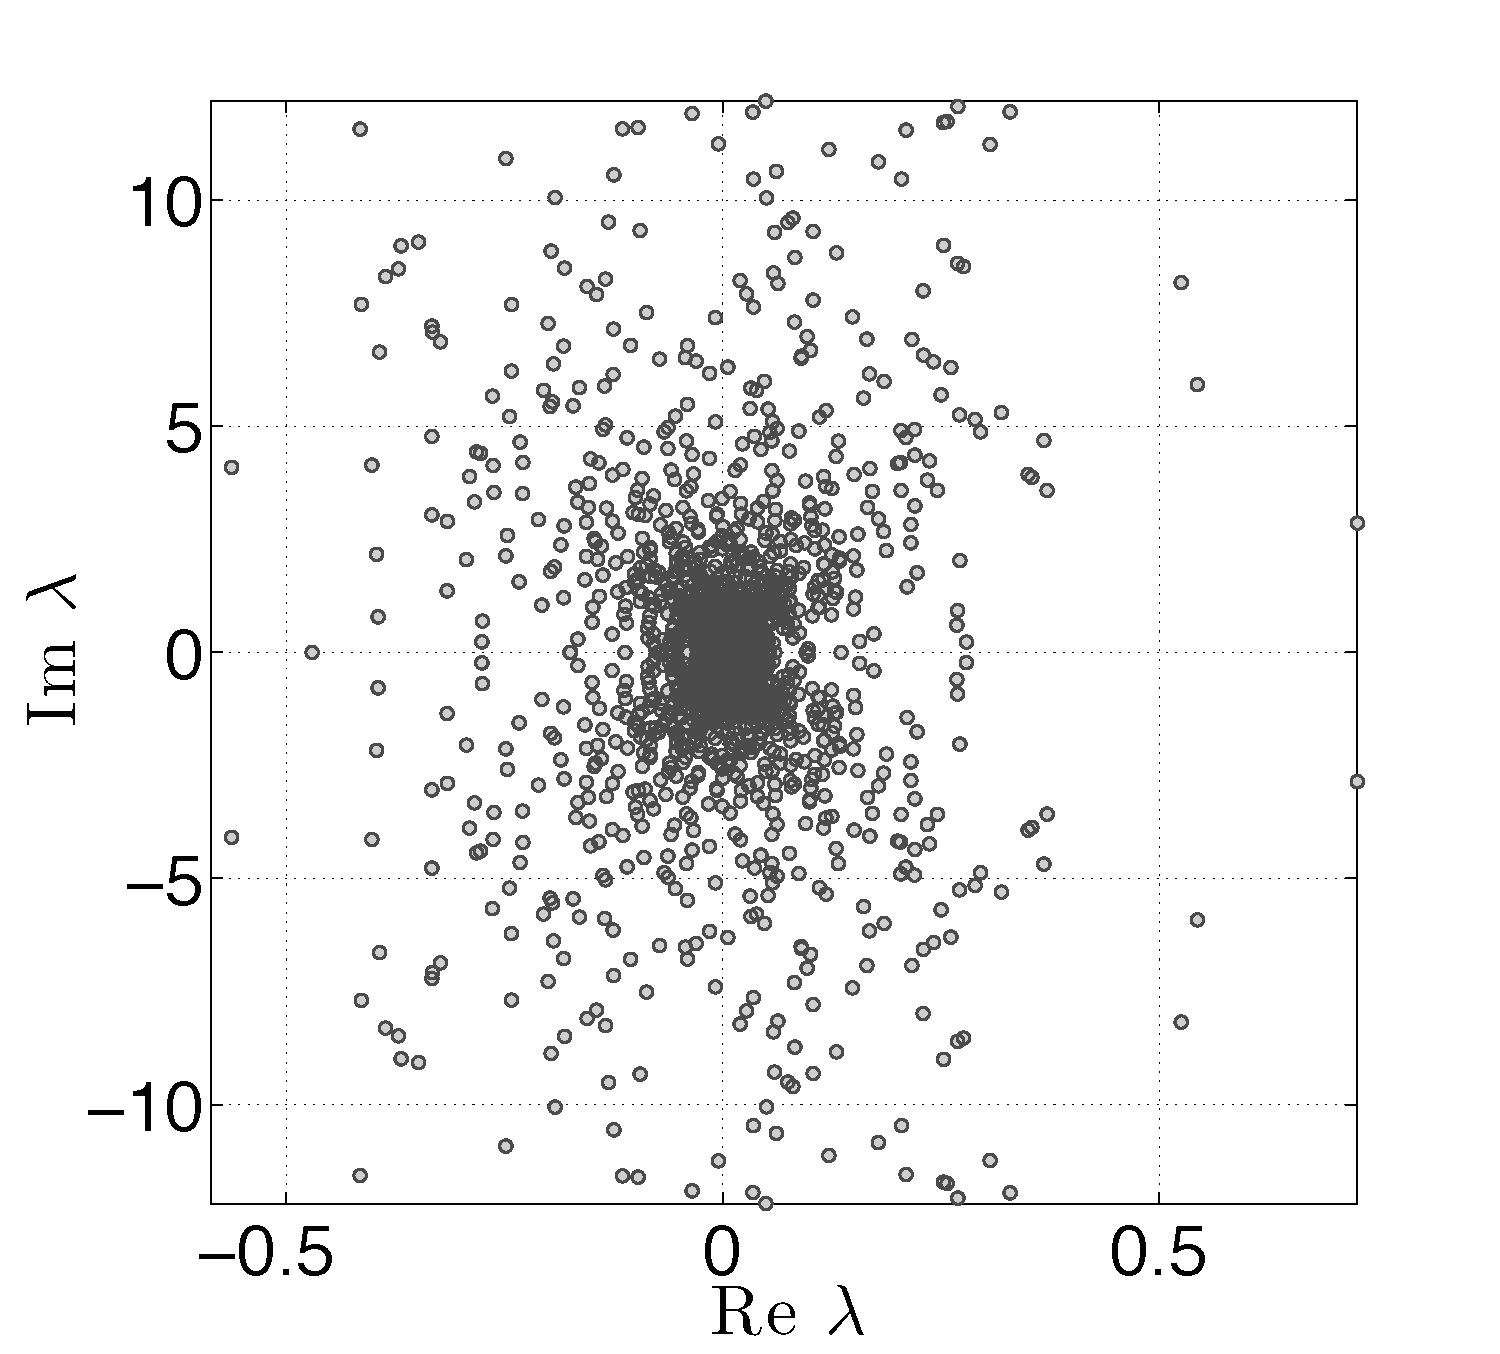
\includegraphics[width=1.0\textwidth]{../figures/paper1/figures/vortex_rollup/eigs_N4096_n101_noHV.pdf}
	\caption{No Hypervsiscosity}
	\label{fig:vortex_eigs_nohv}
\end{subfigure}
\begin{subfigure}[b]{0.45\textwidth}
	\centering
	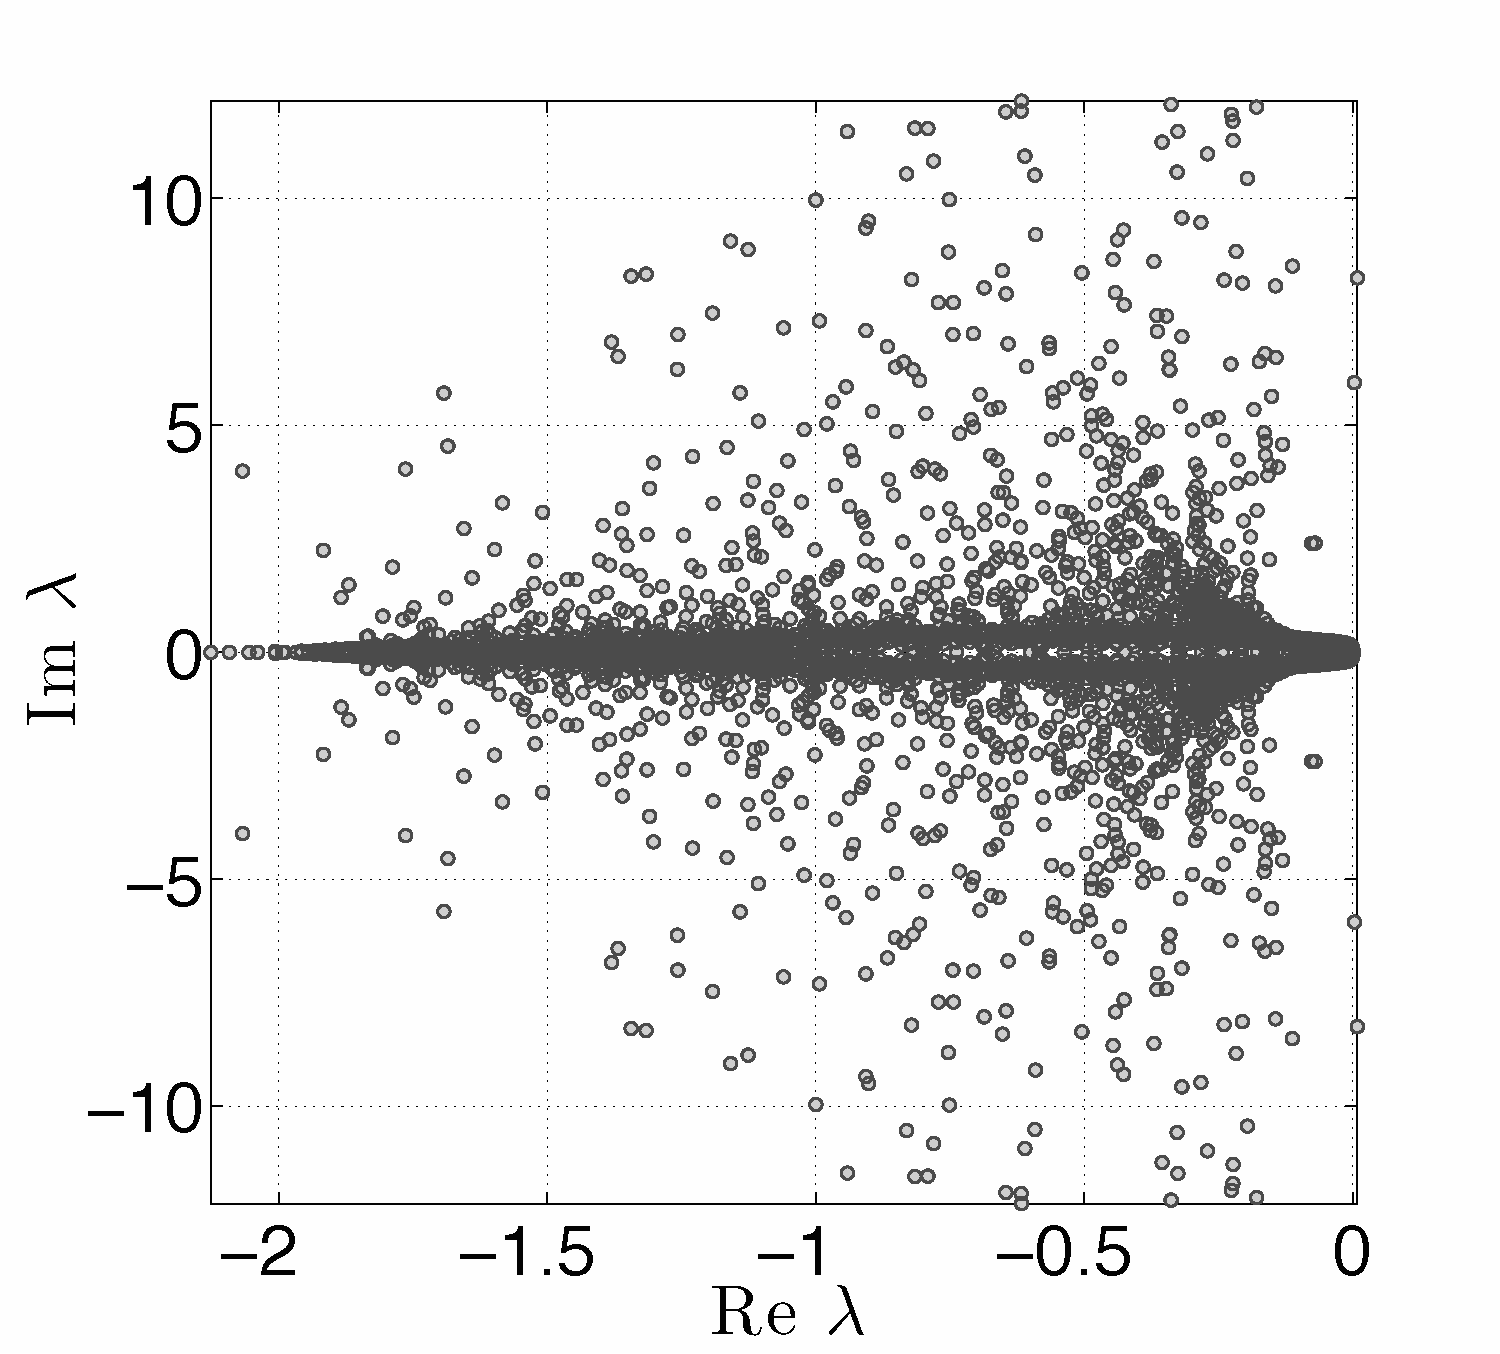
\includegraphics[width=1.0\textwidth]{../figures/paper1/figures/vortex_rollup/eigs_N4096_n101_HV_k4_gamma40.pdf}
	\caption{With Hyperviscosity}
	\label{fig:vortex_eigs_hv}
\end{subfigure}
\caption{Eigenvalues of $\text{diag}(\omega(\theta)) D_\lambda$ for the vortex roll-up test case for $N=4096$ nodes, stencil size $n=101$ and $\epsilon = 3.5$. Left: no hyperviscosity. Right: hyperviscosity enabled with $k=4$ and $\gamma_c = 40$. }
\label{fig:eig_vortex}
\end{center}
\end{figure}

\begin{figure}[htbp]
\begin{center}
\begin{subfigure}[b]{0.45\textwidth}
	\centering
	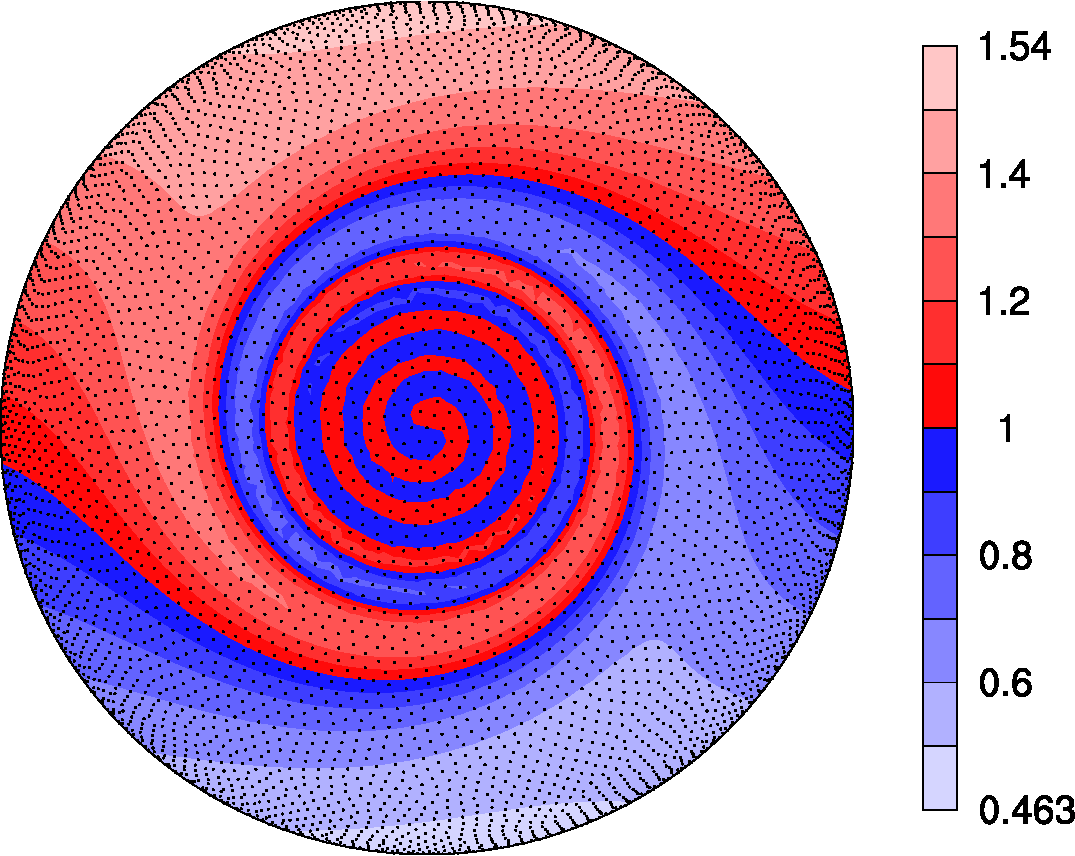
\includegraphics[width=1.0\textwidth]{../figures/paper1/figures/vortex_rollup/vortexComputedSolution-eps-converted-to.pdf}
	\caption{Computed Solution}
	\label{fig:vortex_approx}
\end{subfigure} 
\begin{subfigure}[b]{0.45\textwidth}
	\centering
	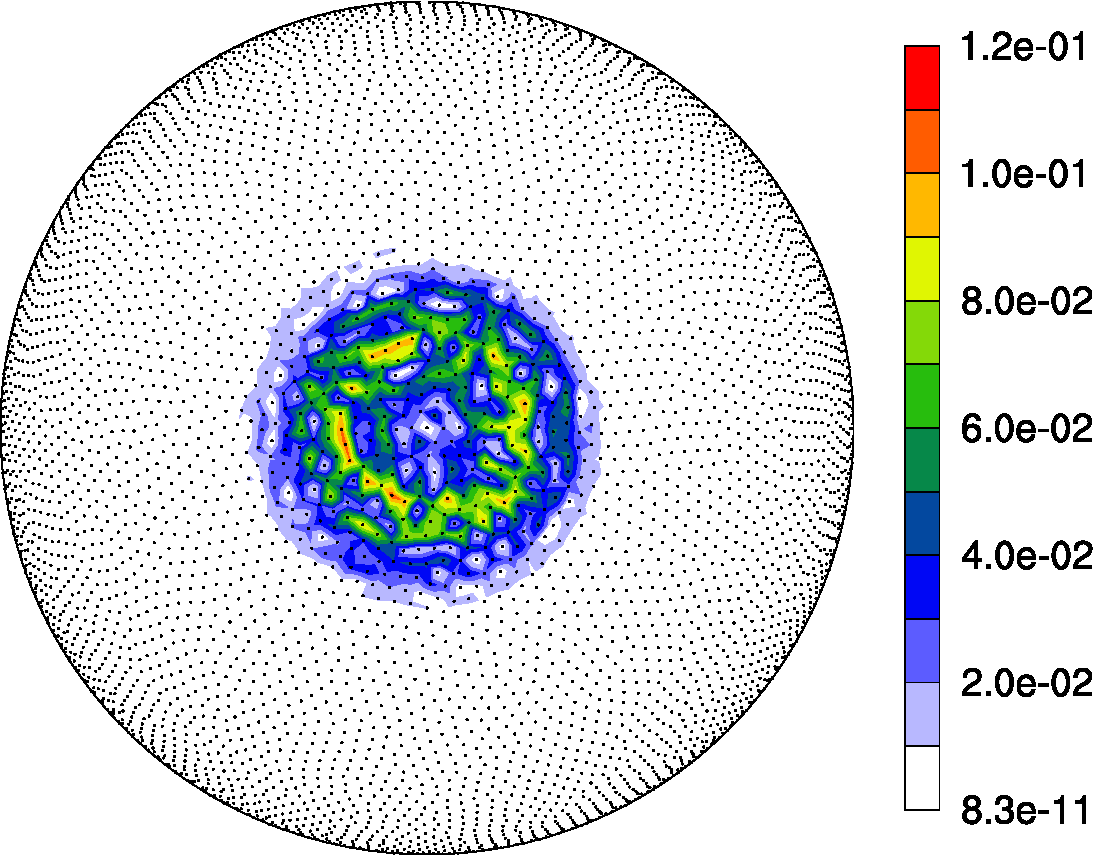
\includegraphics[width=1.0\textwidth]{../figures/paper1/figures/vortex_rollup/vortexRelativeError-eps-converted-to.pdf}
	\caption{Relative Absolute Error}
	\label{fig:vortex_relerr}
\end{subfigure}
\caption{Vortex roll-up solution at time $t=10$ using RBF-FD with $N=10,201$ and $n=50$ point stencil. Normalized $\ell_2$ error of solution at $t=10$ is $1.25(10^{-2})$ \authnote{add initial condition figure} }
\label{fig:vortex_t10}
\end{center}
\end{figure}

Figure~\ref{fig:vortex_t10} shows the solution to Equation~(\ref{eq:vortex}) at $t = 10$, on $N=10201$ nodes, with stencil size $n=50$. This resolution is sufficient to properly capture the vortices at $t=10$, but lower resolutions would suffer approximation errors associated with insufficient grid resolution. 
For this reason, the solution at $t=3$ is considered in the normalized $\ell_2$ error convergence study presented in Figure~\ref{fig:conv_plot_vortex_hv}. The time step $\Delta t = 0.05$ for all resolutions.

\begin{figure}[htbp!]
\begin{center}
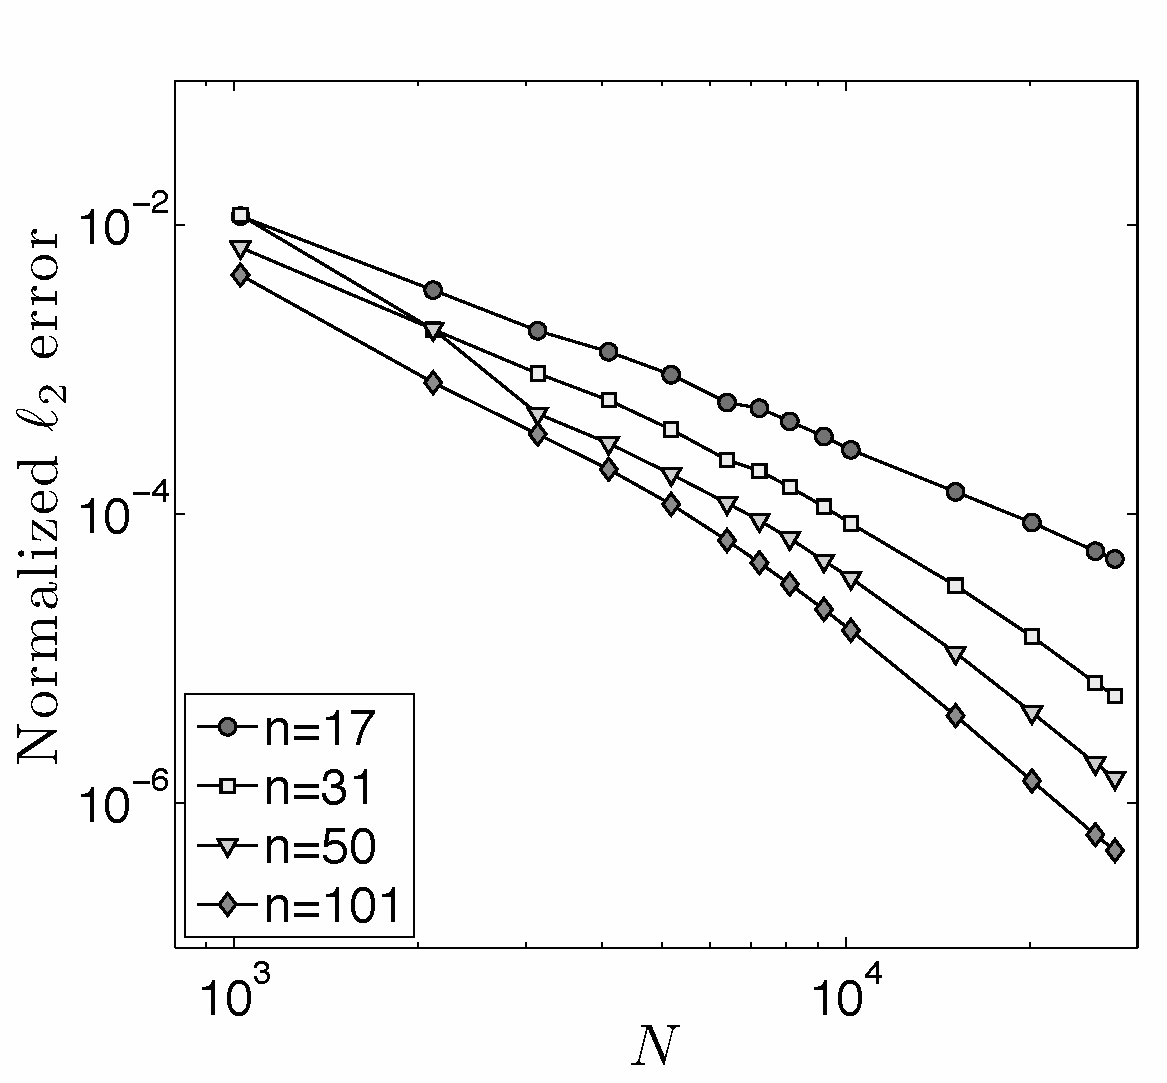
\includegraphics[width=3in] {../figures/paper1/figures/vortex_rollup/convergence_plot_hv.pdf}
\caption{Convergence plot for vortex roll-up at $t=3$. }
\label{fig:conv_plot_vortex_hv}
\end{center}
\end{figure}

% TODO: figures without stabilization
\authnote{Include older figures of convergence without stabilization. Mention that CVT nodes require independent tuning of HV param. Its useful but not incredibly convenient at the moment.}

\subsection{Solid body rotation}

The second test case simulates the advection of a cosine bell over the surface of a unit sphere at an angle $\alpha$ relative to the pole of a standard latitude-longitude grid. The governing PDE is
\begin{equation}
\pd{h}{t} + \frac{u}{\cos \theta} \pd{h}{\lambda} + v \pd{h}{\theta} = 0, \label{eq:cosine_bell}
\end{equation}
with velocity field,
\begin{equation*}
%\begin{cases}
%u =  \cos \theta \cos \alpha + \sin \theta \cos \lambda \sin \alpha,  & \\
%v =  -\sin \lambda \sin \alpha &.
%\end{cases}
\begin{cases}
u =  u_0 (\cos \theta \cos \alpha + \sin \theta \cos \lambda \sin \alpha),  & \\
v =  -u_0(\sin \lambda \sin \alpha) &.
\end{cases}
\end{equation*}
inclined at an angle $\alpha$ relative to the polar axis and velocity $u_0 = 2 \pi / (1036800$ seconds$)$ to require 12 days per revolution of the bell as in \cite{NairTransport05, FlyerWright07}.
%$u_0 = 1$.

The discretized form of (\ref{eq:cosine_bell}) is
\begin{equation}
%D = \text{diag}(\frac{u}{\cos \theta}) D_\lambda + \text{diag}(v) D_\theta
\d{\mathbf{h}}{t} = -\text{diag}\left(\frac{u}{\cos \theta}\right) D_\lambda \mathbf{h} - \text{diag}(v) D_\theta \mathbf{h}
\label{eq:cosine_with_hyperviscosity}
\end{equation}
where DMs $D_\lambda$ and $D_\theta$ contain RBF-FD weights corresponding to all $N$ stencils that approximate $\pd{}{\lambda}$ and $\pd{}{\theta}$ respectively. Rather than merge the differentiation matrices in (\ref{eq:cosine_with_hyperviscosity}) into one operator, our implementation evaluates them as two sparse matrix-vector multiplies. The separate matrix-vector multiplies are motivated by an effort to provide general and reusable GPU kernels. Additionally, they artificially increase the amount of computation compared to the vortex roll-up test case to simulate cases when operators cannot be merged into one DM (e.g., a non-linear PDE).

By splitting the DM, the singularities at the poles ($1 / \cos{\theta} \rightarrow \infty$ as $\theta \rightarrow \pm\frac{\pi}{2}$) in (\ref{eq:cosine_bell}) remain. However, in this case, the approach functions without amplification of errors because the MD node sets have nodes near, but not on, the poles. As noted in \cite{FlyerWright07, FornbergLehto11}, applying the entire spatial operator to the right hand side of Equation~\ref{syst} generates a single DM that analytically removes the singularities at poles. 

We will advect a $C^1$ cosine bell height-field given by
\begin{equation*}
h  =
\begin{cases}
\frac{h_0}{2} (1 + \cos(\frac{\pi \rho}{R}))  & \rho \le R  \\
 0 &  \rho \geq R
\end{cases}
\end{equation*}
having a maximum height of $h_0 = 1$, a radius $R = \frac{1}{3}$ and centered at $(\lambda_c, \theta_c) = (^{3\pi}/_{2}, 0)$, with 
$\rho = \arccos( \sin \theta_{c} \sin \theta + \cos \theta_{c} \cos \theta \cos (\lambda - \lambda_{c}) )$.
The angle of rotation, $\alpha =\ ^{\pi}/_{2}$, is chosen to transport the bell over the poles of the coordinate system.

\begin{table}[ht!]
\caption{Values for hyperviscosity and RBF shape parameter for the cosine bell test. }
\begin{center}
\begin{tabular}{|c|c|c|c|c|c|}
\hline		     & \multicolumn{2}{c|}{$\epsilon = c_1 \sqrt{N} - c_2$} & \multicolumn{2}{c|}{$H = -\gamma_{c} N^{-k} \Delta^{k}$ } \\ \hline
Stencil Size ($n$) & $c_{1}$ & $c_{2}$ & $k$ & $\gamma_c$ \\ \hline
17 & 0.026 & 0.08 & 2 & $8 * 10^{-4}$ \\
31 & 0.035 & 0.1 & 4 & $5 * 10^{-2}$ \\
50 & 0.044 & 0.14 & 6 & $5 * 10^{-1}$ \\
101 & 0.058 & 0.16 & 8 & $5 * 10^{-2}$ \\ \hline
\end{tabular}
\end{center}
\label{tbl:cos_hv_params}
\end{table}

\begin{figure}[ht!]
\begin{center}
\begin{subfigure}[b]{0.45\textwidth}
	\centering
	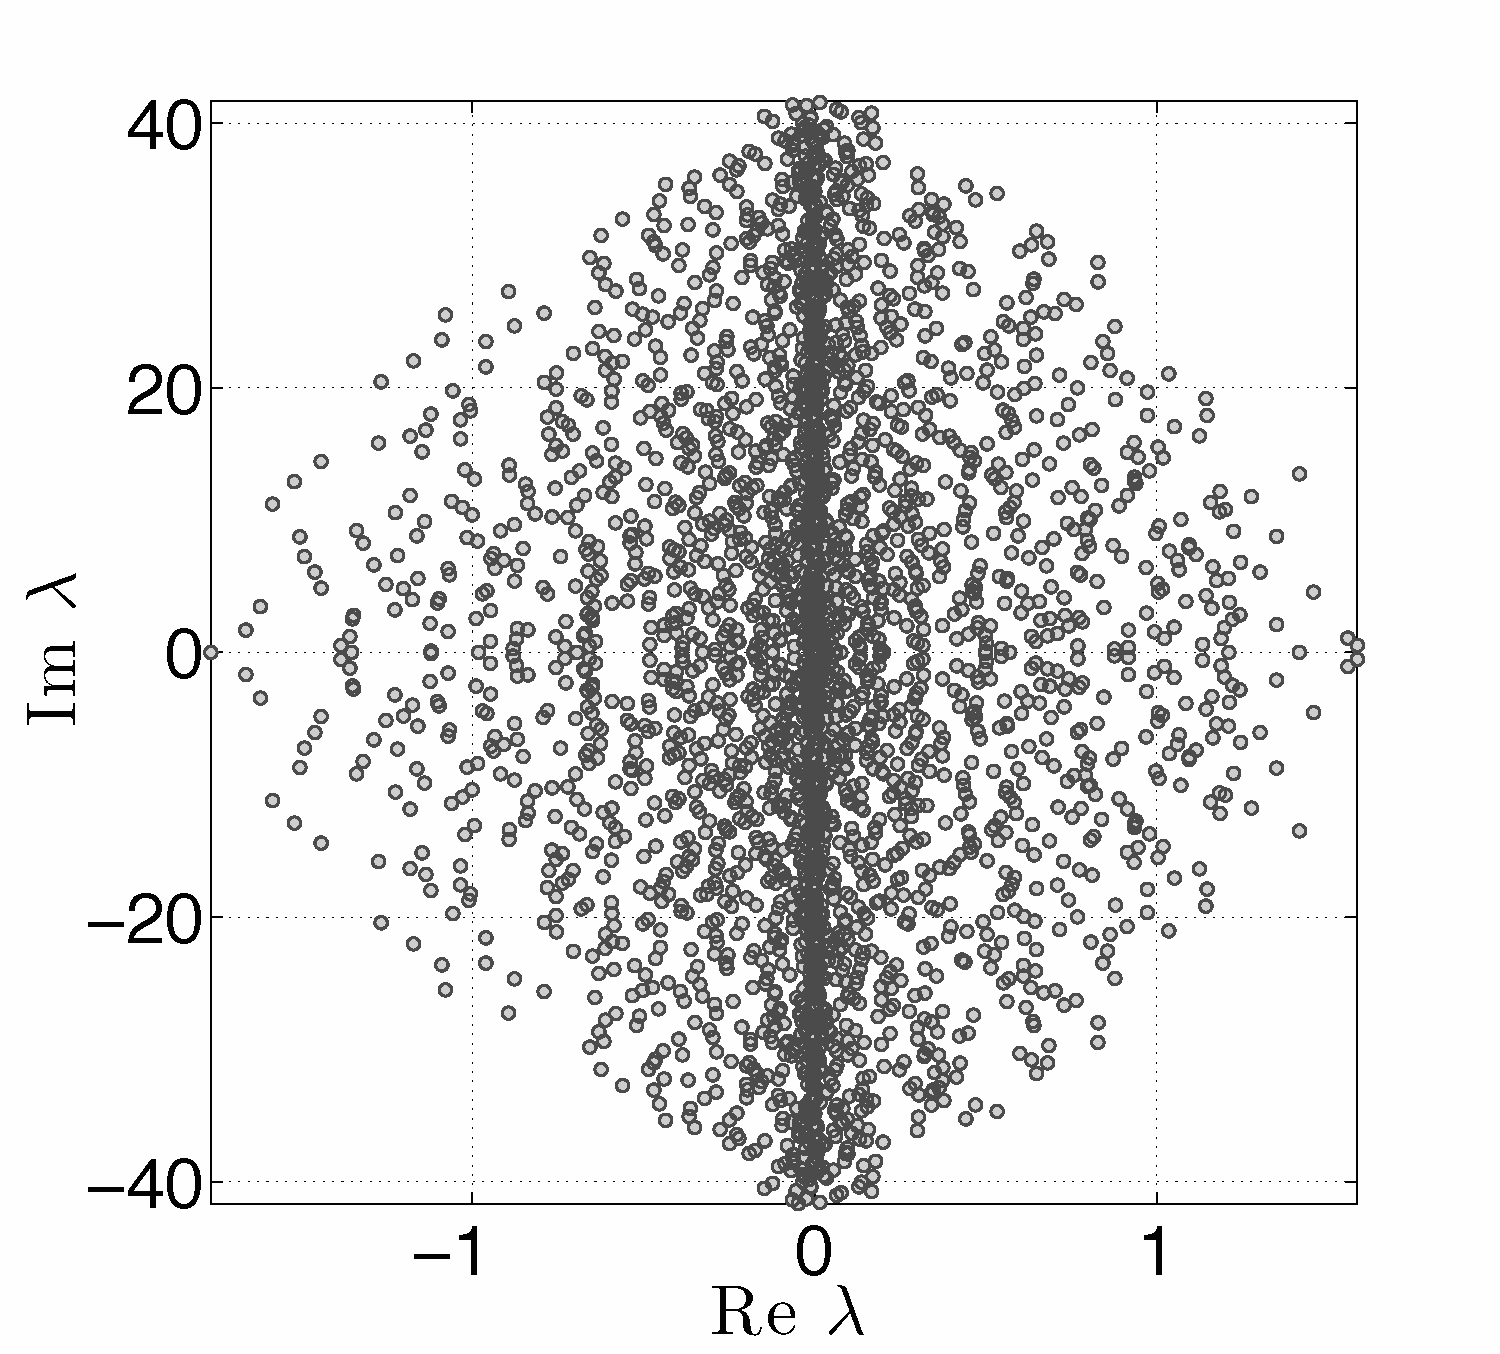
\includegraphics[width=1.0\textwidth]{../figures/paper1/figures/cosine_bell/eigs_N4096_n101_noHV_SCALED.pdf}
	\caption{No Hyperviscosity}
	\label{fig:cosine_eigs_nohv}
\end{subfigure}
\begin{subfigure}[b]{0.45\textwidth}
	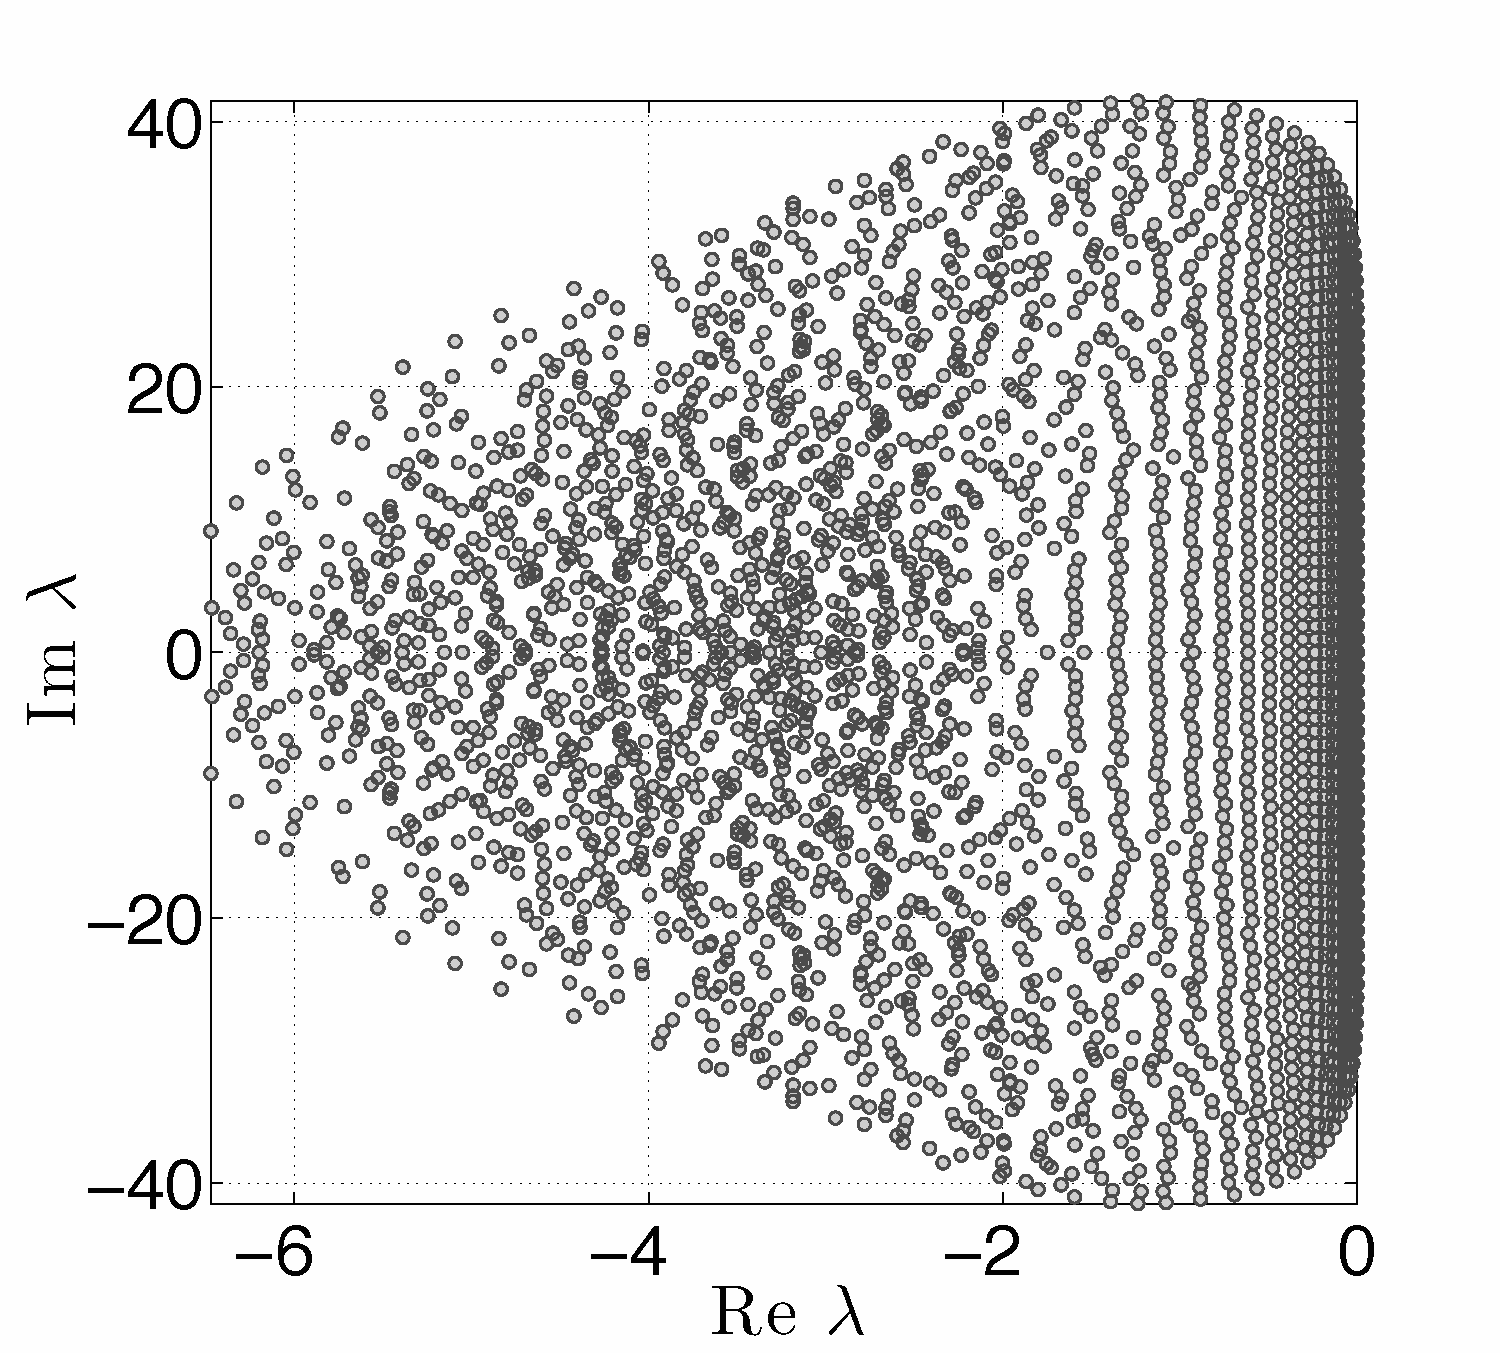
\includegraphics[width=1.0\textwidth]{../figures/paper1/figures/cosine_bell/eigs_HV_N4096_n101_k8_gamma5e_m2_SCALED.pdf}
	\caption{With Hyperviscosity}
	\label{fig:cosine_eigs_hv}
\end{subfigure}
\caption{Eigenvalues of (\ref{eq:cosine_with_hyperviscosity}) for the cosine bell test case with $N=4096$ nodes, stencil size $n=101$, and $\epsilon = 3.5$. Left: no hyperviscosity. Right: hyperviscosity enabled with $k=8$ and $\gamma_c = 5*10^{-2}$. Eigenvalues are divided by $u_0$ to remove scaling effects of velocity.  
}
\label{fig:eig_cosine}
\end{center}
\end{figure}

\begin{figure}[ht!]
\begin{center}
\begin{subfigure}[b]{0.45\textwidth}
	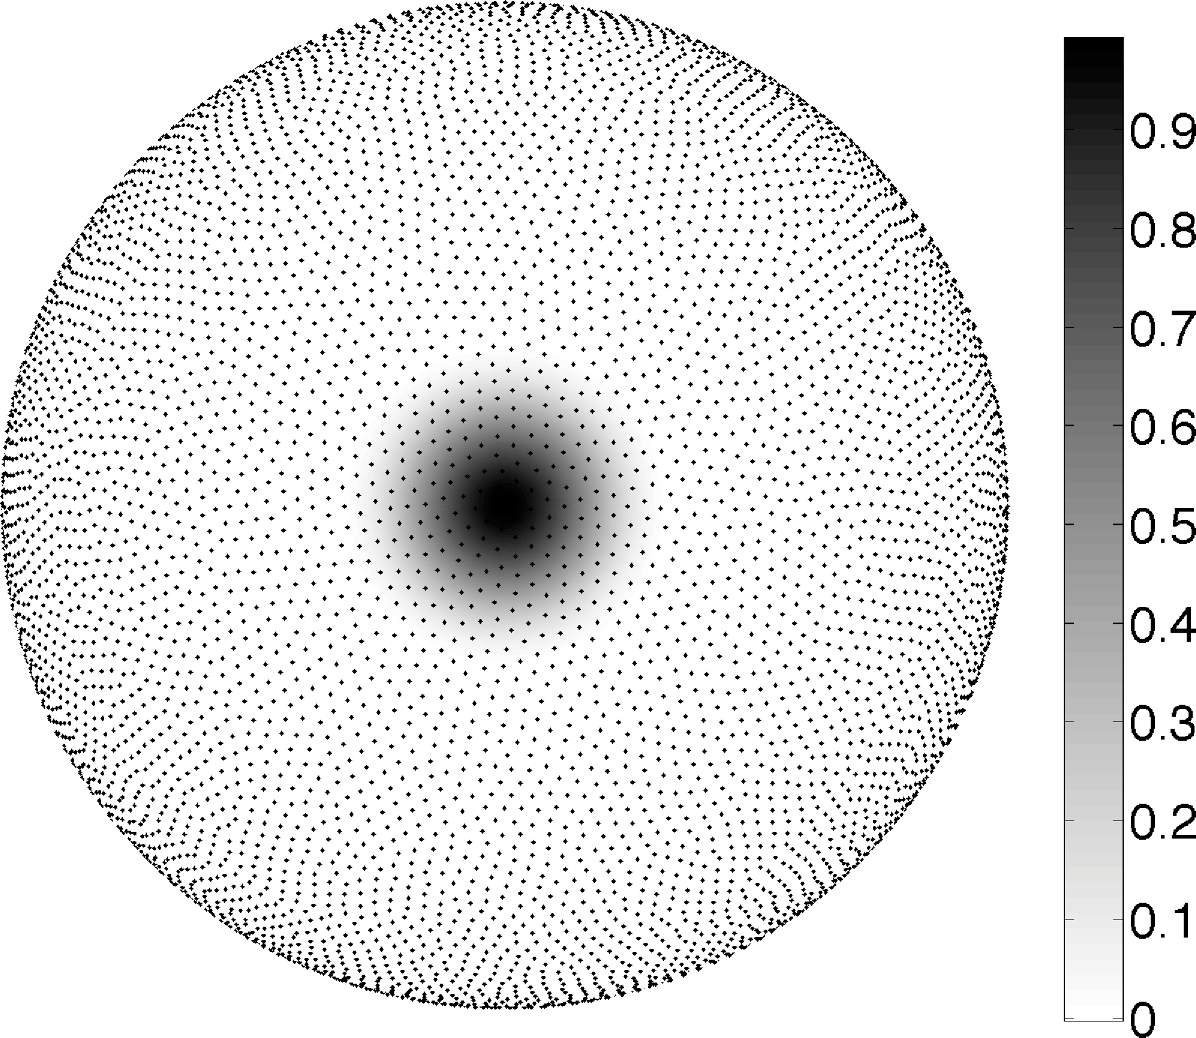
\includegraphics[width=1.0\textwidth]{../figures/paper1/figures/cosine_bell/trimmed_ComputedSolution_ManualBar.pdf}
	\caption{10 Revolutions}
	\label{fig:cosine_approx}
\end{subfigure}
\begin{subfigure}[b]{0.45\textwidth}
	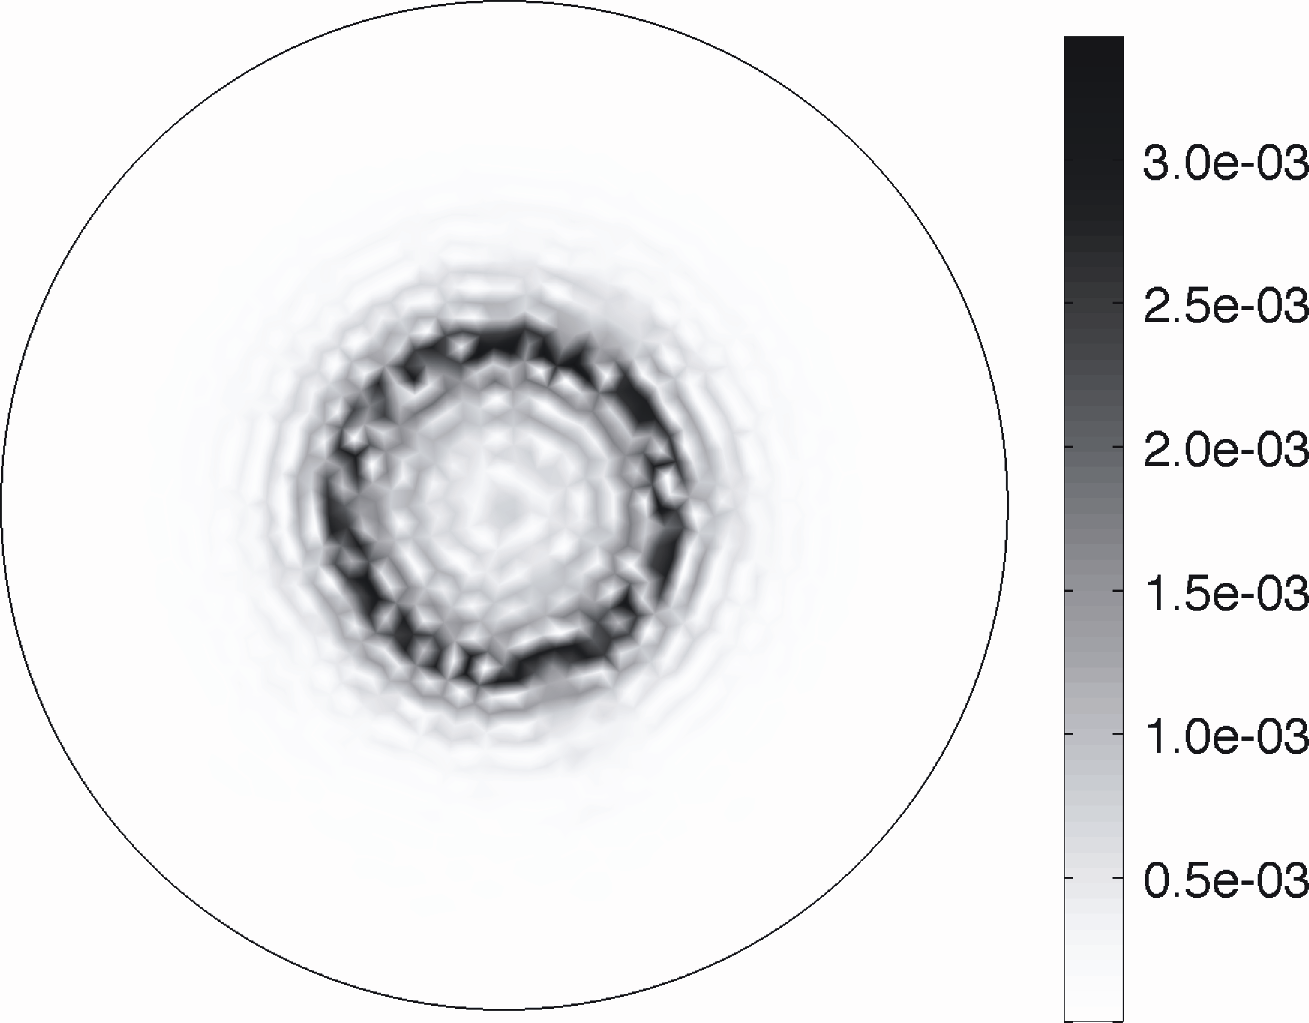
\includegraphics[width=1.0\textwidth]{../figures/paper1/figures/cosine_bell/trimmed_Error_CoveredScale2.pdf}
	\caption{Absolute Error at $10$ Revolutions}
	\label{fig:cosine_abserror}
\end{subfigure}
\caption{Cosine bell solution after 10 revolutions with $N=10201$ nodes and stencil size $n=101$.
Hyperviscosity parameters are $k = 8$, $\gamma_c = 5(10^{-2})$. 
}
 \label{fig:cosine_10revs}
\end{center}
\end{figure}

Figure~\ref{fig:eig_cosine} compares eigenvalues of the DM for $N=4096$ nodes and stencil size $n=101$ before and after hyperviscosity is applied. To avoid scaling effects of velocity on the eigenvalues, they have been scaled by $1/u_0$.  The same approach as in the vortex roll-up case is used to determine the parameters for hyperviscosity and $\epsilon$. Our tuned parameters are presented in 
%\blue{However, note the difference in scale on the real axis compared to the vortex roll-up case; the initial range of the real part of the eigenvalues is approximately four orders of magnitude smaller. In this case, eigenvalues are more sensitive to the hyperviscosity filter. 
Table~\ref{tbl:cos_hv_params}.
% provides appropriate parameters for hyperviscosity in this test case. %, which reflect the difference in scale of $\gamma_c$ compared to Table~\ref{tbl:vortex_hv_params}.
%The parameters for hyperviscosity are dependent on $u_0$ 

%\clearpage

Figure~\ref{fig:cosine_10revs} shows the cosine bell transported ten full revolutions around the sphere. Without hyperviscosity, RBF-FD cannot complete a single revolution of the bell before instability takes over. However, adding hyperviscosity allows computation to extend to dozens or even thousands of revolutions and maintain stability (e.g., see \cite{FornbergLehto11}). After ten revolutions, the cosine bell is still intact. The majority of the absolute error (Figure~\ref{fig:cosine_abserror}) appears at the base of the $C^1$ bell where the discontinuity appears in the derivative. At ten revolutions, Figure~\ref{fig:conv_cosine_bell} illustrates the convergence of the RBF-FD method. All tests in Figure~\ref{fig:conv_cosine_bell} assume 1000 time-steps per revolution (i.e., $\Delta t = 1036.8$ seconds). 


\hl{Complete:}
17.28 minutes was a conservative step that allowed the problem to scale up to $N=27556$ nodes. Compare this to the conservative 30 minute time-step taken for $N=4096$ nodes in \cite{FlyerWright07}, which was already half necessary for DG and 8x less than necessary for both Spherical Harmonics and Double Fourier methods.\authnote{It would be good to quantify the appropriate $dt$ that would compare RBF-FD to their $N=4096$ case with global RBFs.} 


\begin{figure}[htbp]
\begin{center}
% TODO: Color figure
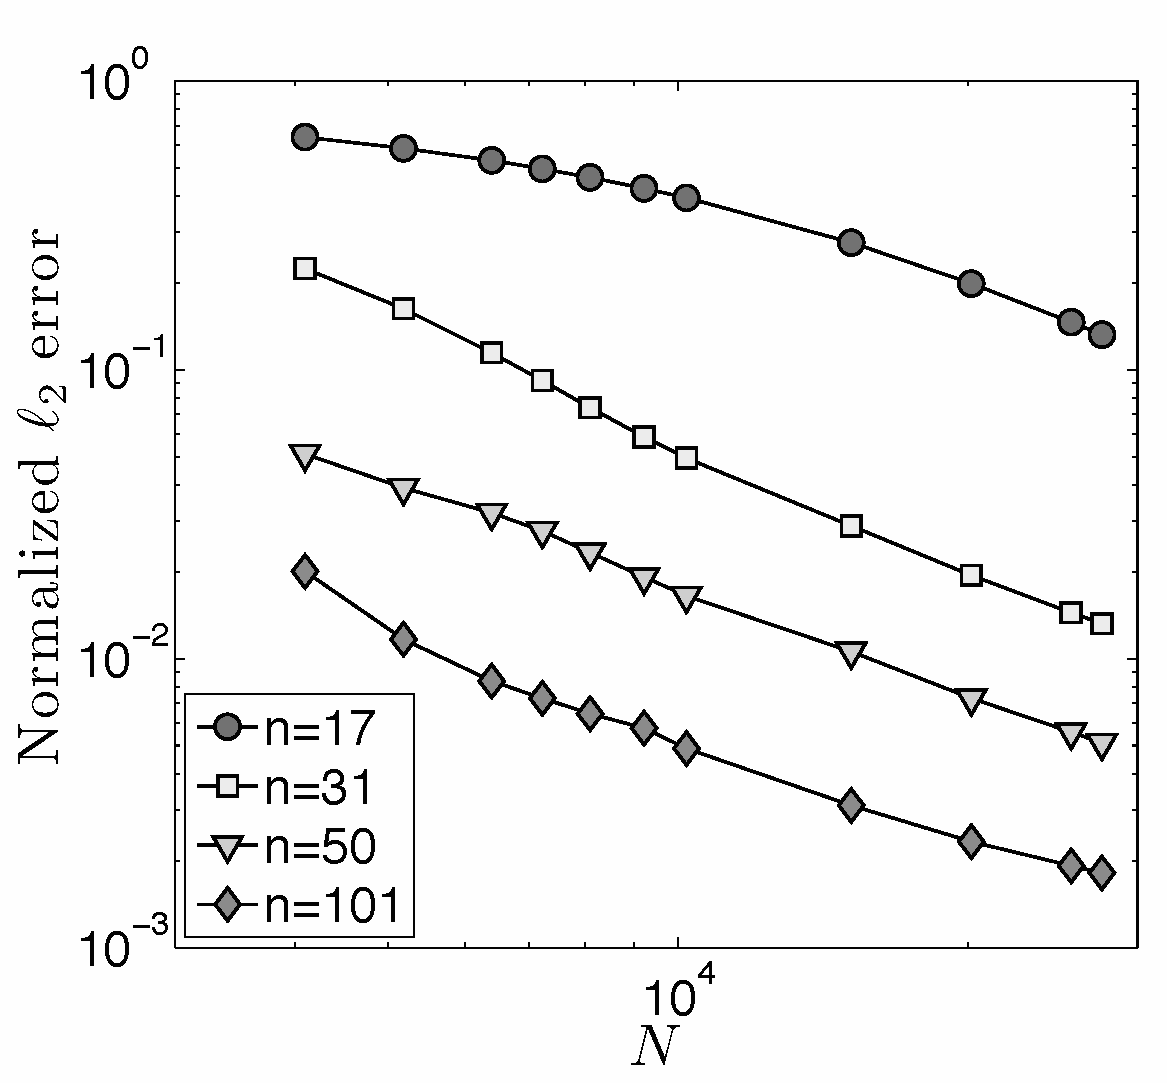
\includegraphics[width=3in]{../figures/paper1/figures/cosine_bell/convergence_plot_hv.pdf}
\caption{Convergence plot for cosine bell advection. Normalized $\ell_2$ error at 10 revolutions with hyperviscosity enabled. }
\label{fig:conv_cosine_bell}
\end{center}
\end{figure}



\section{Fragments (integrate above)}
To verify our multi-CPU and multi-CPU+GPU implementations, two hyperbolic PDEs on the surface of the sphere are tested. For both cases a spherical coordinate system is used in terms of latitude $\lambda$ and longitude $\theta$:
\begin{eqnarray*} 
x & = & \rho \cos \lambda \cos \theta, 	\\
y & = & \rho \sin \lambda \cos \theta, 		\\
z & = & \rho \sin \theta.		
\end{eqnarray*}

Node sets are the Maximum Determinant point distributions on the sphere \cite{Sloan2003} consistent with previously published results (see e.g., \cite{Flyer2007} and \cite{Fornberg2011b}).

Hyperviscosity parameters $\gamma_c$ and $k$ depend on the RHS of the PDE. 
For this test case, hyperviscosity scaling parameters are listed in Table~\ref{tbl:vortex_hv_params}. Linear functions to choose the RBF support parameter $\epsilon$ are also provided. The parameters $\gamma_c$ and $k$ were obtained via trial-and-error parameter searching on $N=4096$ nodes. The goal when choosing parameters is to push all eigenvalues to the left half-plane, and then tweak $\gamma_c$ up or down to condense the eigenvalues as near to the imaginary axis as possible. We try to keep the range of filtered eigenvalue real parts within twice the width of the unfiltered range, so hyperviscosity does not cause too much diffusion in the solution. 

For the cosine bell we use the initial conditions
\begin{equation*}
h  = 
\begin{cases} 
\frac{h_0}{2} (1 + \cos(\frac{\pi \rho}{R})  & \rho \le R  \\
 0 &  \rho \geq R 
\end{cases}
\end{equation*}
where the bell of radius $R = \frac{a}{3}$ is centered at $(\lambda_c, \theta_c)$ and provided by the expression,
\begin{eqnarray*}
\rho = a \arccos( \sin \theta_{c} \sin \theta + \cos \theta_{c} \cos \theta \cos (\lambda - \lambda_{c}) ).
\end{eqnarray*}
We assume $a = 1$, $h_0 = 1$, and $(\lambda_c, \theta_c) = (^{3\pi}/_{2}, 0)$. The angle $\alpha =\ ^{\pi}/_{2}$ is chosen to transport the bell over the poles of the coordinate system, and $u_0 =\ ^{2 \pi a}/_{1036800}$. 

\authnote{State that we can split operator to test cases like nonlinear PDEs.} 

\authnote{Include figures from NCL or Paraview}

\subsection{CFL}
We constrict our timesteps according to the Courant-Friedrich-Lewy (CFL) condition: 

$$
C_{\text{max}} \frac{\Delta x_{\text{min}}}{v_{\text{max}}} < \Delta t
$$
where $\Delta x_{\text{min}}$ is the minimum distance between any two nodes in the domain, and the $v_{\text{max}}$ is the maximum velocity 

For the cosine bell test cases we use a conservative $C_{\text{max}} = 0.4$ to ensure stable transport in all cases with $n=101$. However, in testing it was found that $n=17$ is capable of stably advecting with $C_{\text{max}} > 1$ for $n=17$; $n=101$ can go up to $C_{\text{max}} = 0.51$ for $N=27556$ (e.g. 650 timesteps per revolution). 


apparently, canceling the cosine analytically causes the conditioning of the system to change slightly. The hyperviscosity parameters I have in the paper are for the case with the cosine present. The parameters continue to function well for the other cases, but their impact on the eigenvalue distributions is noticeably higher (further span to the left). 


\section{GFLOP Throughput}
In order to quantify the performance of our implementation, we can measure two
factors. First, we can check the speedup achieved on the GPU relative to the
CPU to get an idea of how much return of investment is to be expected by all
the effort in porting the application to the GPU. Speedup is measured as the
time to execute on the CPU divided by the time to execute on the GPU. 

The second quantification is to check the throughput of the process. By
quantifying the GFLOP throughput we have a measure that tells us two things:
first, a concrete number quantifying the amount of work performed per second by
either hardware, and second because we can calculate the peak throughput possible on
each hardware, we also have a measure of how occupied our CPU/GPU units are.
With the GFLOPs we can also determine the cost per watt for computation and
conclude on what problem sizes the GPU is cost effective to target and use. 

Now, as we parallelize across multiple GPUs, these same numbers can come into
play. However we are also interested in the efficiency. Efficiency is the
speedup divided by the number of processors. With efficiency we have a measure
of how well-utilized processors are as we scale either the problem size (weak)
or the number of processors (strong). As the efficiency diminishes we can
conclude on how many stencils/nodes per processor will keep our processors
occupied balanced with the shortest compute time possible (i.e., we are
maximizing return of investment). 


\ifstandalone
\bibliographystyle{plain}
\bibliography{merged_references}
\end{document}
\else
\expandafter\endinput
\fi


